% 学習結果説明（手順5a：温度シフト構造の見直し。用語集と図の見方）
% results フォルダで「lualatex 学習結果説明_手順5a.tex」を2回実行すると PDF を作り直せる（TeX Live の LuaLaTeX を使用）。
% 図は results/step5a/ の PNG を相対パスで読み込む。
\documentclass[paper=a4paper,fontsize=10.5pt,line_length=44zw,number_of_lines=38]{jlreq}
\usepackage[haranoaji]{luatexja-preset}
\usepackage{amsmath}
\usepackage{graphicx}
\usepackage{booktabs}
\usepackage{tabularx}
\usepackage{enumitem}
\usepackage{float}
\usepackage{xcolor}
\usepackage[hidelinks,bookmarksnumbered]{hyperref}
\graphicspath{{step5a/}}

\newcommand{\file}[1]{\texttt{\detokenize{#1}}}
\newcommand{\gd}{\dot{\gamma}}
\newcommand{\Tff}{T_{\mathrm{ff}}}
\newcommand{\Tset}{T_{\mathrm{set}}}
\newcommand{\Eh}{E_{\mathrm{h}}}
\newcommand{\Ev}{E_{\mathrm{v}}}
\newenvironment{termlist}{\begin{itemize}[label=・,leftmargin=1\zw,labelwidth=1\zw,labelsep=0pt,itemsep=0.4ex,topsep=0.6ex,parsep=0pt]}{\end{itemize}}
\newcommand{\term}[1]{\item \textbf{#1}：}
\newenvironment{points}{\begin{itemize}[label=$\triangleright$,leftmargin=1.5\zw,itemsep=0.3ex,topsep=0.5ex,parsep=0pt]}{\end{itemize}}
\newcommand{\pt}[1]{\item \textbf{#1}：}
\newcommand{\ptn}[1]{\item \textbf{#1}}
\renewcommand{\arraystretch}{1.25}

\title{樹脂粘度モデル開発　手順5aの学習結果の説明\\[0.6ex]{\large 温度シフト構造の見直し：用語集とグラフの見方（機械学習・統計を初めて学ぶ人向け）}}
\author{}
\date{2026年10月14日}

\begin{document}
\maketitle
{\small\tableofcontents}

% =====================================================================
\section{この文書について}

この文書は、\file{results/step5a/} にある手順5aの結果（図と表）を、機械学習や統計を初めて学ぶ人でも読めるように説明したものです。手順3a・3b の説明書（\file{学習結果説明_手順3a.pdf}・\file{学習結果説明_手順3b.pdf}）と同じ形で、重なる用語は短く繰り返しています。

\begin{points}
\pt{対象の結果}\file{results/step5a/}：粘度の温度依存性を、どんな式で組み込むのがよいかを比べた結果です（図 10 枚、CSV 9 個）。
\pt{読み方}2章で「なぜ見直すのか」と「何を比べたか」をつかみ、分からない言葉は3章の用語集で調べてください。4章で図の見方、5章で表の見方、6章で結果のまとめと、構造の決定（本命 B・対案 A）を説明します。
\pt{数値について}文中の数値は、この文書を作った時点の results の表から取り出したものです。
\pt{決定}ユーザーの決定（2026-10-12）で、構造は\textbf{本命 B（横・縦を別々）、対案 A（縦だけ）}に改めました（6.2節）。後で自分で実行して比べられるように、ノートに両者を並べて見る節（ノートの8章。本書の表\ref{tab:main}）を作りました。
\pt{記号表}記号・モデル名・列名の一覧は、\file{学習結果説明_記号表.pdf} にあります（この文書の記号も含みます）。
\pt{元のノート}\file{01_機械学習コードフォルダ} の \file{手順5a_シフト構造の見直し.ipynb} です。設定を変えるときは、ノートの「設定エリア」だけを直します。報告書・発表資料用の高解像度のグラフ（せん断速度 ― 粘度）は、ノート末尾のセルで作ります（4.8節）。
\pt{作り直し方}\file{results} フォルダで \texttt{lualatex 学習結果説明\_手順5a.tex} を2回実行すると、この PDF を作り直せます。
\end{points}

% =====================================================================
\section{何をしたか（概要）}

\subsection{なぜ見直すのか}
当初の計画（CLAUDE.md §5）では、「溶融温度（加熱シリンダの設定温度 $\Tset$）を、時間–温度換算則のシフトとして組み込む」構造を考えていました。樹脂の粘度は、温度を上げると下がります。高分子の溶融体には、「温度を変えると、粘度とせん断速度の関係（流動曲線）が、形を変えずに、横（せん断速度）と縦（粘度）にずれるだけ」という性質（時間–温度換算則）があるとされます。そのずれの大きさを、温度の関数（シフトファクター $a_T$）として決めれば、1つの曲線（マスターカーブ）から、どの温度の粘度も予測できます。

当初の構造は、横方向と縦方向のずれを、同じ活性化エネルギー $E$ で決める形でした。

\begin{equation}
\ln\eta = \ln a_T(E) + f\bigl(\ln\gd + \ln a_T(E),\ \ln \mathrm{Fo}\bigr),\qquad \ln a_T = \frac{E}{R}\Bigl(\frac1T - \frac1{T_{\mathrm{ref}}}\Bigr)
\end{equation}

ところが、新データの試算では、この形では最適な $E$ が 0 付近か負になり、文献値の目安（PP の流動で 40 kJ/mol 前後）は、データと大きく合いませんでした。理由は、見かけの流動曲線の傾き $s = d\ln\eta/d\ln\gd$ が約 $-1.6$ と急で（せん断速度が上がると、せん断応力が下がる）、同じせん断速度での粘度の差が $(1+s)\,\Delta\ln a_T$ になるためです。$E>0$ にすると「低温ほど粘度が低い」予測になり、データ（低温ほど高い）と逆になります。手順5aは、構造を見直して、データに合う形を探すための手順です。

\subsection{データと分け方}
\begin{points}
\pt{データ}手順3a・3bと同じです（外れ値なし。PP は、問題データ一覧の「除外」を除いたもの）。条件ごとに、ショットの $\ln\eta$ と $\ln\gd$ を平均した「条件平均」を、尤度の比較に使います（5data は 93 条件）。
\pt{S\_V}5data で学習し、3data で検証する（射出速度の両端への外挿）。低速側（3・5 mm/s）と高速側（280・320 mm/s）に分けて評価します。
\pt{S\_T}5data の 190・230 ℃ だけで学習し、210 ℃ を全部テストにします（設定温度の内挿）。3data の 210 ℃ は S\_T3 として別に評価します（速度の外挿も重なります）。
\pt{ALL}5data と 3data をまとめたデータ（129 条件）。最終的な $E$ の推定値を見るために使います。
\end{points}

\subsection{比べた構造}
\begin{table}[H]
\caption{比べた構造。$u = \ln\gd + \ln a_T(\Eh)$、$\mathrm{Fo}$ はフーリエ数（冷却の度合い。$\ln\mathrm{Fo} = -(\ln\gd + 3\ln H) + $ 定数）}
\begin{tabularx}{\linewidth}{@{}l>{\raggedright\arraybackslash}p{12\zw}X@{}}
\toprule
記号 & 式 & 意味 \\
\midrule
H & $\ln\eta = \ln a_T(E) + f(u,\ln\mathrm{Fo})$、$\Eh=\Ev=E$ & 当初の構造（§5）。温度を変えると、流動曲線が横にも縦にも、同じ割合でずれる。 \\
A & $\ln\eta = \ln a_T(\Ev) + f(\ln\gd,\ln\mathrm{Fo})$ & 曲線の形は変えず、縦（粘度）だけを、一定の倍率でずらす。 \\
Hz & $\ln\eta = f(u,\ln\mathrm{Fo})$ & 曲線の形は変えず、横（せん断速度）だけをずらす。 \\
B（本命） & $\ln\eta = \ln a_T(\Ev) + f(u,\ln\mathrm{Fo})$ & 横と縦を、別々の $E$ でずらす。A の一定の倍率に、条件で変わる分が加わる。 \\
N & H の $E=0$ & 温度を無視する（ずらさない）基準。 \\
H40 & H で $E=40$ kJ/mol に固定 & 文献値の目安を当てはめた確認。 \\
F & H と同じ式で、$T$ に $\Tff$ を使う & 参考。$\Tff$ は流動の結果で、事前には分からない。 \\
C & $\ln\eta = f(\ln\gd,\ln H,\Tset)$ & 比較の基準。構造なしで、$\Tset$ を普通の入力に並べた GPR。 \\
\addlinespace
\multicolumn{3}{@{}l}{\small 「何が表せるか」「なぜ採用したか」「結果」は、表のすぐ下の2.3.1節に、構造ごとに書きました。} \\
\bottomrule
\end{tabularx}
\end{table}

$f$ はガウス過程（GPR。ARD 付き Matern 5/2 に線形カーネルとノイズを足したもの）です。$R = 8.314$ J/mol/K、基準温度 $T_{\mathrm{ref}} = 210$ ℃ です。

\subsubsection{それぞれの形で、何が表せるか（なぜ採用したか）}
表1の「構造」は、\textbf{温度を変えたとき、流動曲線（横軸 $\gd$、縦軸 $\eta$ の対数グラフの曲線）がどう動くか}を式にしたものです。曲線の動き方には、\textbf{横にずれる}（同じ粘度になるせん断速度が変わる）と、\textbf{縦にずれる}（同じせん断速度での粘度が変わる）の2通りがあります。構造の違いは、「どちらを、どれだけずらすか」の違いです。図\ref{fig:concept}（4章）に、形の違いの模式図（実データではない）を付けました。以下、構造ごとに、「この形で何が表せるか」「なぜ採用したか（何を期待したか）」「結果はどうだったか」を書きます。

\begin{points}
\ptn{H：横も縦も同じ割合でずらす（当初の構造）}
  \begin{itemize}[leftmargin=1.5\zw,itemsep=0.2ex,topsep=0.2ex,parsep=0pt]
  \item \textbf{表せること}：温度を変えると、曲線の形は変わらず、横と縦に、同じ割合 $a_T$ だけずれる。基準温度（210 ℃）の曲線を1本決めれば、$E$ という1つの数で、ほかの温度の曲線がすべて決まる（図\ref{fig:concept}の左端）。
  \item \textbf{採用した理由と期待}：高分子の溶融体で広く成り立つとされる時間--温度換算則（Cross-WLF モデルも、この考え方）をそのまま使う形。温度ごとのデータを1本のマスターカーブにまとめられるので、水準の少ない設定温度でも温度依存性を表せること、$E$ を文献値（PP の流動で 40 kJ/mol 前後）と比べて、データの妥当性も確かめられることを期待した。
  \item \textbf{結果}：期待どおりにならなかった。見かけの傾き $s$ が約 $-1.6$ と急なため、横にずらした分の粘度の差が、逆向きに効く。最良の $E$ は学習データごとに動き（PP：$-$10.5, $-$3.0, 7.5 kJ/mol）、LML も温度なしと大差ない（差 6・11）。
  \end{itemize}
\ptn{A：縦だけずらす（対案）}
  \begin{itemize}[leftmargin=1.5\zw,itemsep=0.2ex,topsep=0.2ex,parsep=0pt]
  \item \textbf{表せること}：曲線の形は温度で変わらず、全体が一定の倍率で上下に動く。同じせん断速度で、低温ほど粘度が一定の倍率だけ高い。190 ℃ と 230 ℃ の粘度の比は $\exp(0.0207\,\Ev)$（図\ref{fig:concept}の2列目）。
  \item \textbf{採用した理由と期待}：実測の「190 ℃ の粘度は 230 ℃ の 1.1〜1.2 倍」を、パラメータ1個（$\Ev$）で、いちばん簡単に表せる形。H が失敗したのは、横のずらしが傾きと組み合わさって向きが逆になるためなので、横のずれを外して、縦のずれだけを残した。
  \item \textbf{結果}：$\Ev$ は PP で 7.5、粉砕材混合 PP で 7.5 kJ/mol と、学習データによらず同じ値に決まる。LML は温度なしより 73・70 大きく、検証の精度は通常の GPR（C）と同等。ただし、倍率が厚みによらず一定なので、実測の「厚いほど温度の効果が大きい」は表せない。
  \end{itemize}
\ptn{Hz：横だけずらす}
  \begin{itemize}[leftmargin=1.5\zw,itemsep=0.2ex,topsep=0.2ex,parsep=0pt]
  \item \textbf{表せること}：曲線の形も高さも変わらず、全体が横にだけ動く。同じ粘度になるせん断速度が、温度で変わる（図\ref{fig:concept}の3列目）。
  \item \textbf{採用した理由と期待}：対照。「横のずれだけで、温度の効果を表せるか」を確かめる。
  \item \textbf{結果}：$\Eh$ が負（PP：$-$7.0, $-$4.5, $-$4.0、粉砕材混合 PP：$-$6.5, $-$4.5, $-$6.5 kJ/mol）に決まり、「低温ほど、同じ粘度になるせん断速度が大きい」ことになって、物理的に解釈しにくい。LML も A に劣る。
  \end{itemize}
\ptn{B：横と縦を別々にずらす（本命）}
  \begin{itemize}[leftmargin=1.5\zw,itemsep=0.2ex,topsep=0.2ex,parsep=0pt]
  \item \textbf{表せること}：A の「一定の倍率の上下」に、横のずれを足した形。流動曲線の傾きは、せん断速度や厚みで違う（傾きが急な所では、横にずらしたときの粘度の変化が大きい）ので、同じ温度差でも、条件ごとに粘度の比が変わる。「厚いほど（低せん断の側ほど）、温度の効果が大きい」を表せる（図\ref{fig:concept}の右端）。
  \item \textbf{採用した理由と期待}：A の分かりやすさ（$\Ev$ が土台）を残したまま、A が表せなかった厚み依存を足せる。H（$\Eh=\Ev$）と A（$\Eh=0$）を特別な場合として含むので、データがどれを支持するかを、$\Eh$・$\Ev$ の値で確かめられる。
  \item \textbf{結果}：LML が最大（A より 78・54 大きい）で、厚みごとの粘度の比（実測は 0.5 mm で約 1.08、2.0 mm で約 1.19）も再現する。ただし、$\Eh$ と $\Ev$ は別々には決めきれず、差 $\Ev-\Eh$（約 9 kJ/mol）だけが決まる（図2）。
  \end{itemize}
\ptn{N・H40・F・C：比べるための基準}
  \begin{itemize}[leftmargin=1.5\zw,itemsep=0.2ex,topsep=0.2ex,parsep=0pt]
  \item N は温度を無視する基準（$E=0$）、H40 は文献値 $E=40$ kJ/mol を当てはめたときの確認、F は $\Tff$ でずらす参考（$\Tff$ は流れの結果で、事前には分からない）。C は構造を入れず、$\Tset$ を普通の入力として GPR に並べたもの。\textbf{構造あり（A・B）が C と同等以上の精度なら、構造がデータで支持された}、とみなす（CLAUDE.md §6）。
  \end{itemize}
\end{points}

\subsection{$E$ の決め方（プロファイル尤度）}
$E$ を格子（1 次元は 2.5 kJ/mol 刻み、B は 5 kJ/mol 刻み）で振り、それぞれの $E$ で、入力と出力を換算して GPR を学習し、\textbf{対数周辺尤度}（LML：データがそのモデルでどれだけ「ありそう」か。大きいほどよい）を求めます。LML が最大になる $E$ を採用します。最良の点の近くは、さらに細かい格子（1 次元は 0.5 kJ/mol、B は 1 kJ/mol 刻み）で計算し直します。

注意点が3つあります。(1) 出力の自動標準化は使いません（$E$ ごとに尺度が変わり、LML を比べられなくなるため）。入力の標準化も、$E$ に依存しない定数で行います。(2) 尤度の比較は、条件平均で行います。ショットごとの $\gd$ を入力にすると、$E\ne 0$ のとき設定温度が入力の上で少し分かれ、GPR がそれを温度の目印に使えてしまうためです。(3) 予測の評価では、決めた $E$ を使い、ショット単位の GPR を学習し直します。入力の $\gd$ は、条件平均（cm。成形条件から見た予測）とショットごと（shot）の両方で調べました。

% =====================================================================
\section{用語集}

「・用語：説明」の形で、手順3a・3bの用語集になかったものを中心に並べました。

\subsection{温度シフトに関する用語}
\begin{termlist}
\term{時間–温度換算則（TTS）}温度を変えると、流動曲線が形を変えずにずれるだけ、という経験則。温度を上げることと、ゆっくり流すことが「同じ効果」を持つ、という意味で、時間（せん断速度）と温度を換算できます。
\term{シフトファクター $a_T$}曲線をどれだけずらすかを表す係数。基準温度で 1。温度が低いほど大きくなります（粘い、遅い）。
\term{アレニウス型}シフトファクターを $\ln a_T = (E/R)(1/T - 1/T_{\mathrm{ref}})$ で表す形。結晶性の樹脂（PP など）によく使われます。$T$ は絶対温度 [K]。
\term{活性化エネルギー $E$ [kJ/mol]}温度による粘度の変わりやすさを表す量。大きいほど、温度で粘度が大きく変わります。PP の流動では、40 kJ/mol 前後が目安とされます。$E = 40$ kJ/mol なら、190 ℃ の粘度は 230 ℃ の約 2.3 倍になります。1 kJ/mol あたり約 2.1\% 増える計算です（190 ℃ と 230 ℃ の比。$\exp(0.0206\,E)$）。
\term{基準温度 $T_{\mathrm{ref}}$}シフトの基準にする温度（ここでは中間の 210 ℃）。ここで $a_T = 1$。
\term{横方向のシフトと縦方向のシフト}流動曲線を、横軸（せん断速度）の向きにずらすのが横シフト、縦軸（粘度）の向きにずらすのが縦シフトです。時間–温度換算則では、両方を同じ $a_T$ でずらします（式(1)）。
\term{マスターカーブ}シフトで換算した後の、すべての温度のデータを重ねた1本の曲線。温度が違うデータが重なれば、その構造でシフトできています。
\term{見かけの流動曲線の傾き $s$}$\ln\eta$ を $\ln\gd$ に対して描いたときの傾き。$-1$ なら、せん断応力（$\eta\gd$）が一定。$-1$ より急な（$s<-1$）と、せん断速度が上がるほどせん断応力が下がります。新データは約 $-1.6$ で、せん断発熱・冷却・固化の影響を含んだ「見かけ」の値です。同じ $\gd$ での粘度の差は $(1+s)\Delta\ln a_T$ になるので、$s<-1$ だと向きが逆になります。
\term{フーリエ数 $\mathrm{Fo}$}冷却の度合いを表す数。$\alpha\Delta t/H^2$（$\alpha$ は熱拡散率）で、薄いほど、遅いほど大きい。定数は GP に影響しないので、入力は $\ln\mathrm{Fo} = -(\ln\gd + 3\ln H)$ ＋ 定数 を使います。
\end{termlist}

\subsection{推定と評価に関する用語}
\begin{termlist}
\term{対数周辺尤度（LML）}データが、そのモデルのもとでどれだけ「ありそう」かを表す値。大きいほど、データによく合います。パラメータの数が違うモデルでも、公平に比べられます。差が 2〜3 を超えれば、はっきりした違いです。
\term{プロファイル尤度}1つのパラメータ（ここでは $E$）だけを動かし、残りのパラメータはそのつど最適にしたときの LML。$E$ と LML の関係の図（尤度曲線）から、$E$ がどれくらい決まっているかが分かります。山が鋭いほど、$E$ がデータでよく決まっています。
\term{尤度比と「1.92」}LML が最大から 1.92 以内の範囲は、おおよそ 95\% 信頼区間にあたります（尤度比検定の目安）。
\term{条件平均}条件ごとに、ショットの値を平均した値。ショット間のばらつきの影響が小さくなります。
\term{通常の GPR（C）}シフトの構造を入れず、$\ln\gd$・$\ln H$・$\Tset$ を、自由な入力として並べた GPR。構造つきがこれと同等以上なら、構造がデータで支持されたと判断します（CLAUDE.md §6）。
\term{RMSE・被覆率・NLPD}手順3aの用語集と同じです。RMSE は予測の平均的な誤差（$\ln\eta$）、被覆率は 95\% 予測区間に実測が入った割合、NLPD は予測の当たり具合と区間の適切さをまとめた指標（小さいほどよい）。
\term{感度確認}問題データ一覧の P02（190 ℃・0.5 mm・20 mm/s）を学習から除いて、結果がどれだけ変わるかを見ること。
\end{termlist}

% =====================================================================
\section{図の見方}

図ごとに、「何を示す図か」「軸と記号」「見るポイント」「今回の結果」の順に説明します。図の番号は、ファイル名に合わせて 0 から数えます。

\subsection{図0：構造の考え方（模式図）}
\setcounter{figure}{-1}
\begin{figure}[H]
\centering
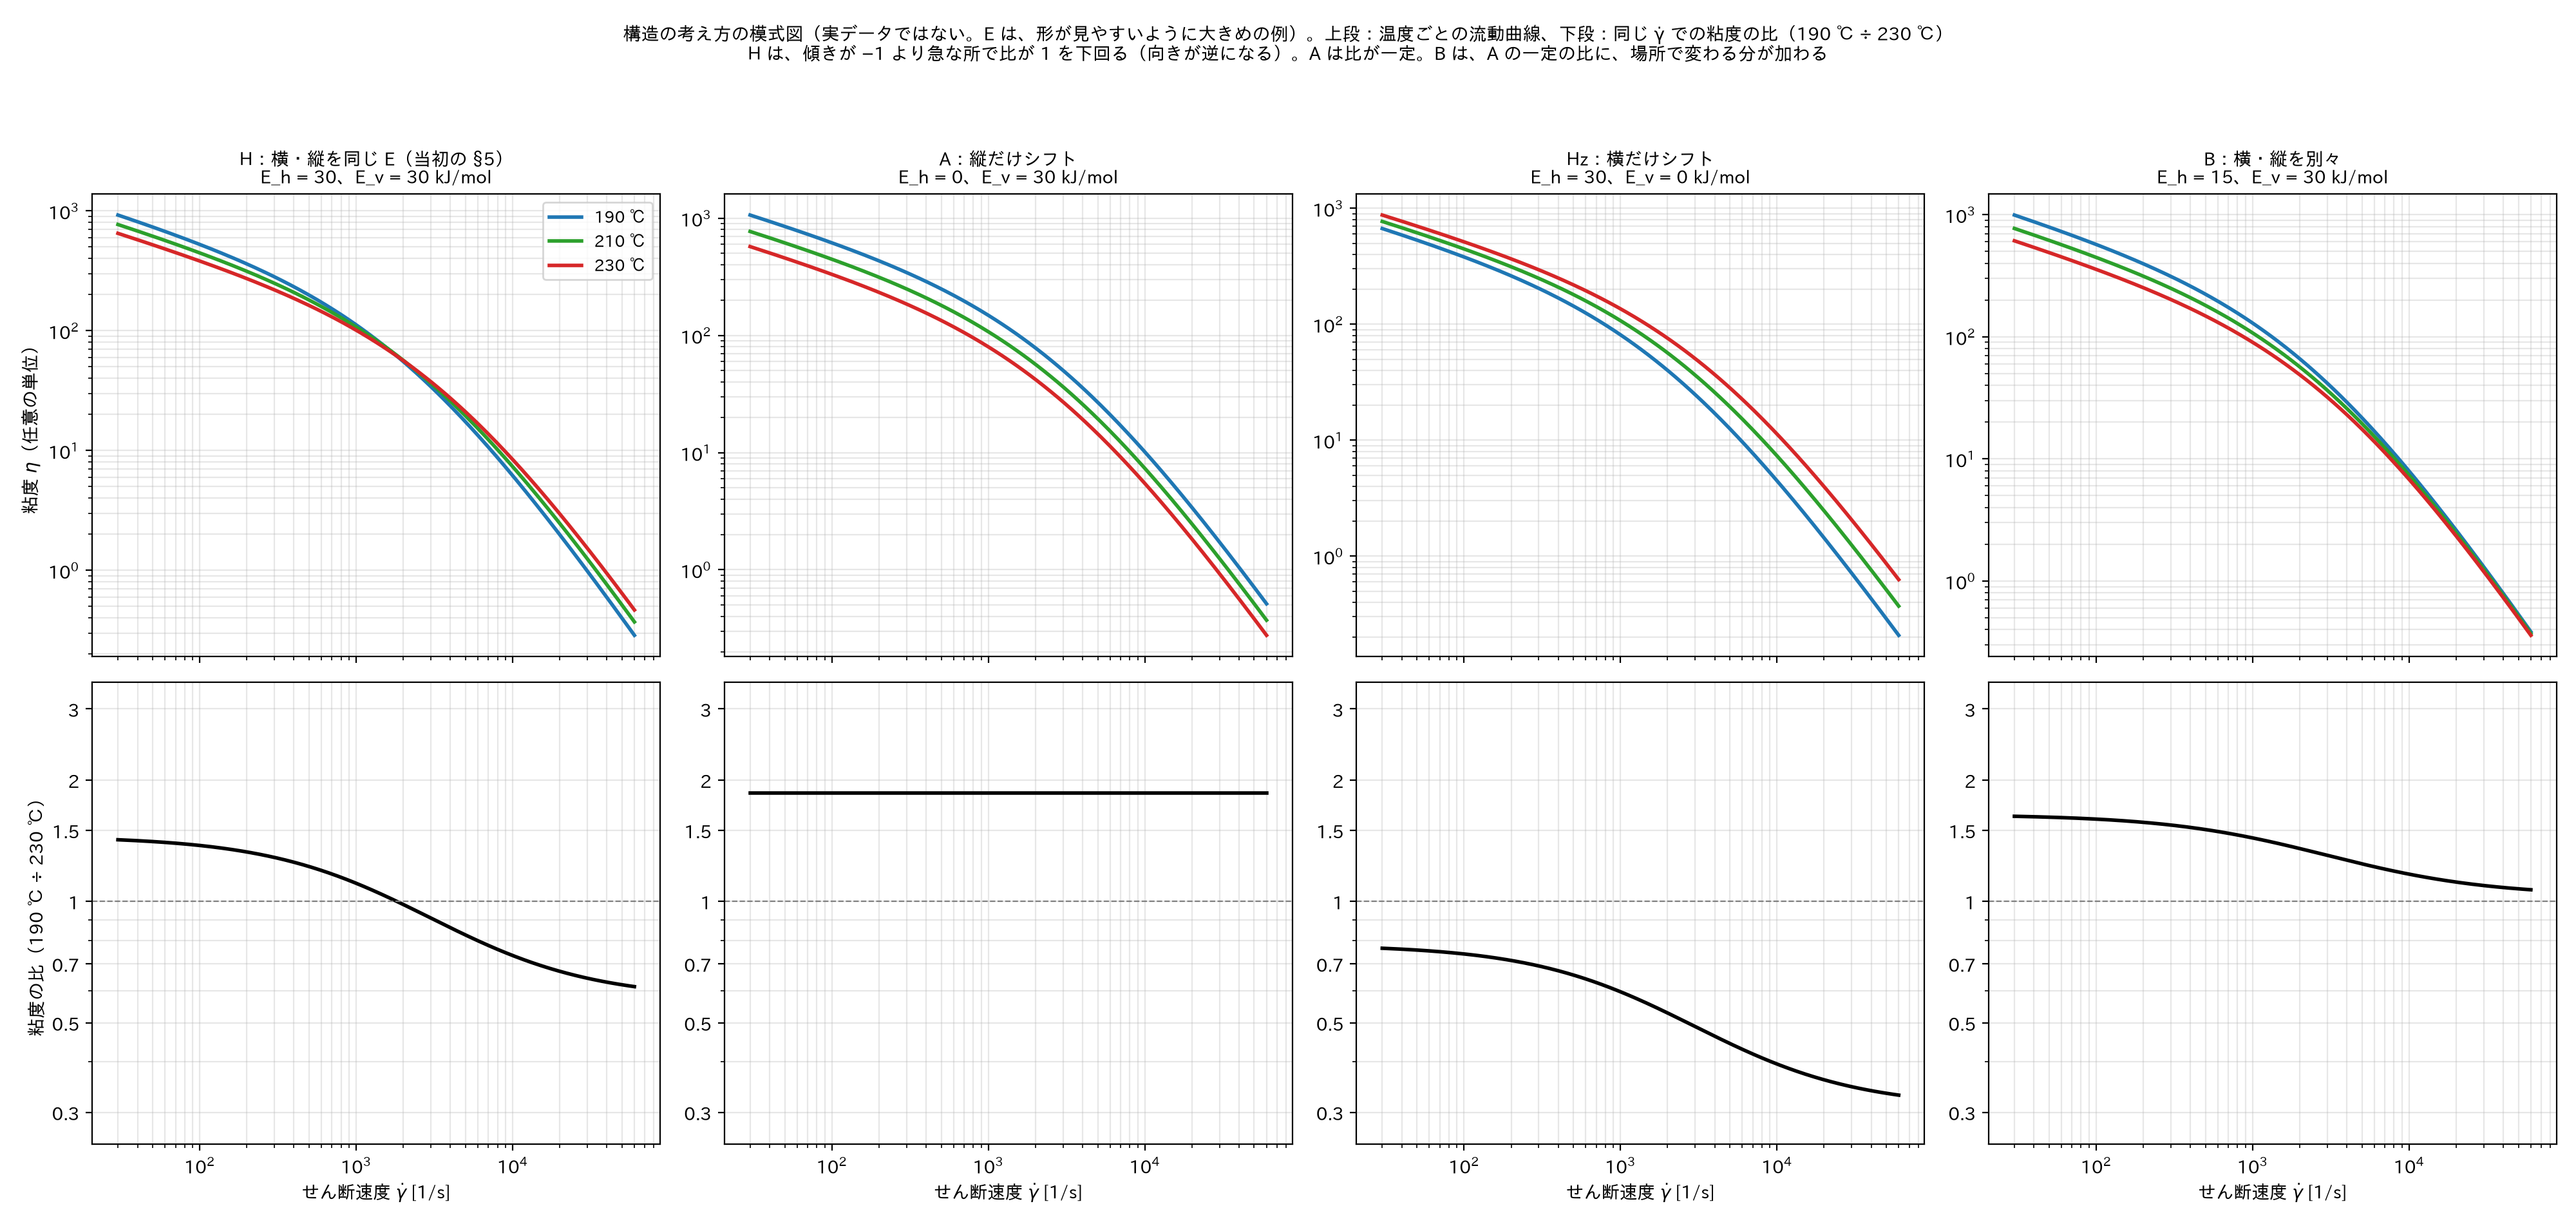
\includegraphics[width=\linewidth]{fig0_shift_concept.png}
\caption{構造の考え方の模式図（実データではない）。上段：温度ごとの流動曲線、下段：同じ $\gd$ での粘度の比（190 ℃ ÷ 230 ℃）}\label{fig:concept}
\end{figure}
\begin{points}
\pt{ファイル}\file{results/step5a/fig0_shift_concept.png}
\pt{何を示す図か}構造 H・A・Hz・B のそれぞれで、温度を変えると流動曲線がどう動くかを、同じ基準の曲線から作って並べた模式図です。実データではありません。形が見やすいように、$E$ は実測より大きめの例（H・A・Hz は 30 kJ/mol、B は $\Eh=15$・$\Ev=30$ kJ/mol）にしました。基準の曲線は、傾きが低せん断で $-0.4$、高せん断で $-1.9$ になる、なめらかな曲線です（見かけの流動曲線は、せん断速度とともに急になります）。
\pt{軸と記号}上段は、横軸が $\gd$、縦軸が $\eta$（任意の単位。対数軸）。青 190 ℃、緑 210 ℃、赤 230 ℃。下段は、横軸が $\gd$、縦軸が同じ $\gd$ での粘度の比（190 ℃ ÷ 230 ℃）で、点線が比 = 1（温度の効果なし）です。
\pt{見るポイント}下段の線が、(1) 1 より上か下か（低温のほうが粘いか）、(2) 水平か（比が一定か）、(3) $\gd$ とともにどう動くか。
\pt{結果の読み方}H：低せん断では比が 1 を超えるが、傾きが $-1$ より急になる高せん断で 1 を下回る（向きが逆になる）。新データの傾きは $-1.6$ 前後なので、H は実測（低温ほど粘い）と合わない。A：比が一定（水平）。B：A の一定の比に、場所で変わる分が加わる（右下がり）。Hz：比が 1 を下回る側に大きく動く。
\end{points}

\subsection{図1：プロファイル尤度（1 次元）}
\begin{figure}[H]
\centering
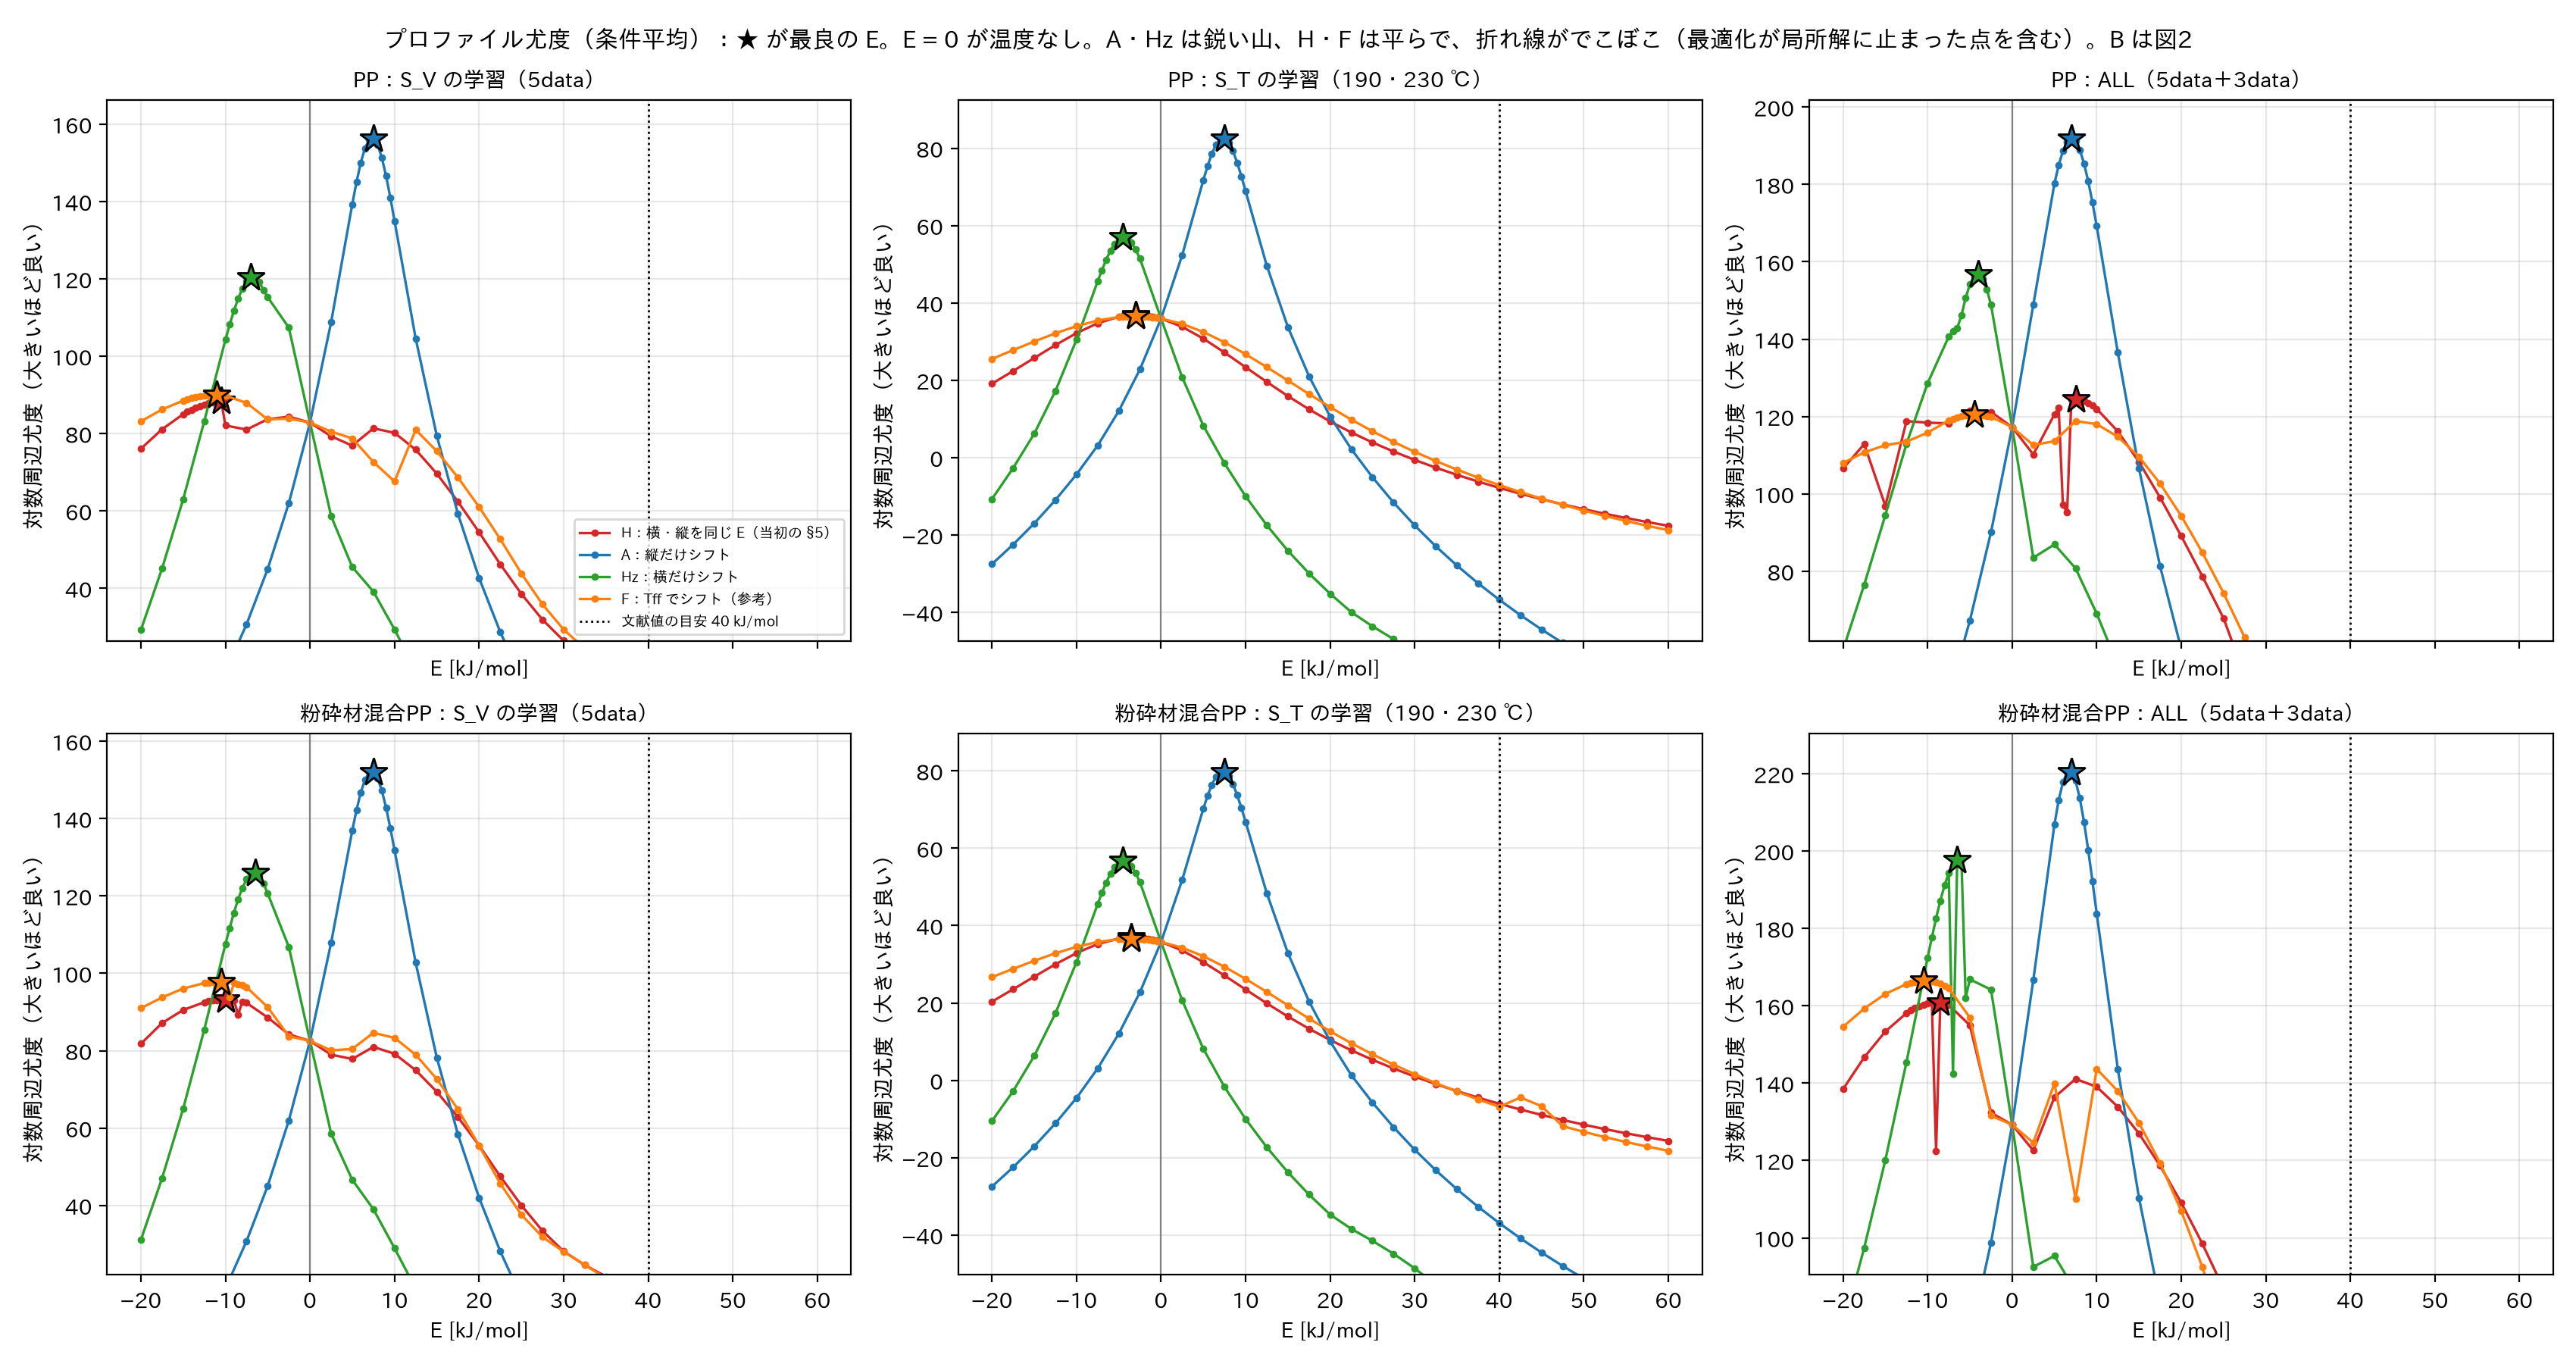
\includegraphics[width=\linewidth]{fig1_profile_likelihood.png}
\caption{構造ごとの、$E$ と対数周辺尤度の関係}
\end{figure}
\begin{points}
\pt{ファイル}\file{results/step5a/fig1_profile_likelihood.png}
\pt{何を示す図か}$E$ を動かしたときの LML を、構造ごとに描いた図です。上段が PP、下段が粉砕材混合 PP。列は学習データ（S\_V の学習、S\_T の学習、ALL）です。
\pt{軸と記号}横軸が $E$ [kJ/mol]、縦軸が LML（大きいほど良い）。色が構造（赤 H、青 A、緑 Hz、橙 F）、★ が各構造の最良の点、縦の灰色の線が $E=0$（温度なし）、黒い点線が文献値の目安 40 kJ/mol です。
\pt{見るポイント}(1) 山が $E=0$ より、どれだけ高いか（温度を入れる意味があるか）。(2) 山が鋭いか平らか（$E$ がデータで決まるか）。(3) 山が 40 kJ/mol の近くにあるか。(4) 学習データを変えても、山の位置が同じか。
\pt{今回の結果}A（縦だけ）は、どの学習データでも鋭い山で、最良の $\Ev$ は PP で 7.5、粉砕材混合 PP で 7.5 kJ/mol（S\_V の学習）、$E=0$ より LML が 73・70 大きくなります。H（当初の構造）は、山が平らで、折れ線もでこぼこです（最適化が局所解に止まった点を含みます）。最良の $E$ は、S\_V・S\_T・ALL の学習で、PP が $-$10.5, $-$3.0, 7.5、粉砕材混合 PP が $-$10.0, $-$3.5, $-$8.5 kJ/mol と、学習データごとに動きます。$E=0$ との LML の差も、S\_V の学習で 6・11 しかありません。$E=40$ では、最良より 75・77 も下がります。Hz（横だけ）は、$E$ が負の側に鋭い山があります。B は図2で見ます。
\end{points}

\subsection{図2：B（横・縦を別々）の 2 次元プロファイル}
\begin{figure}[H]
\centering
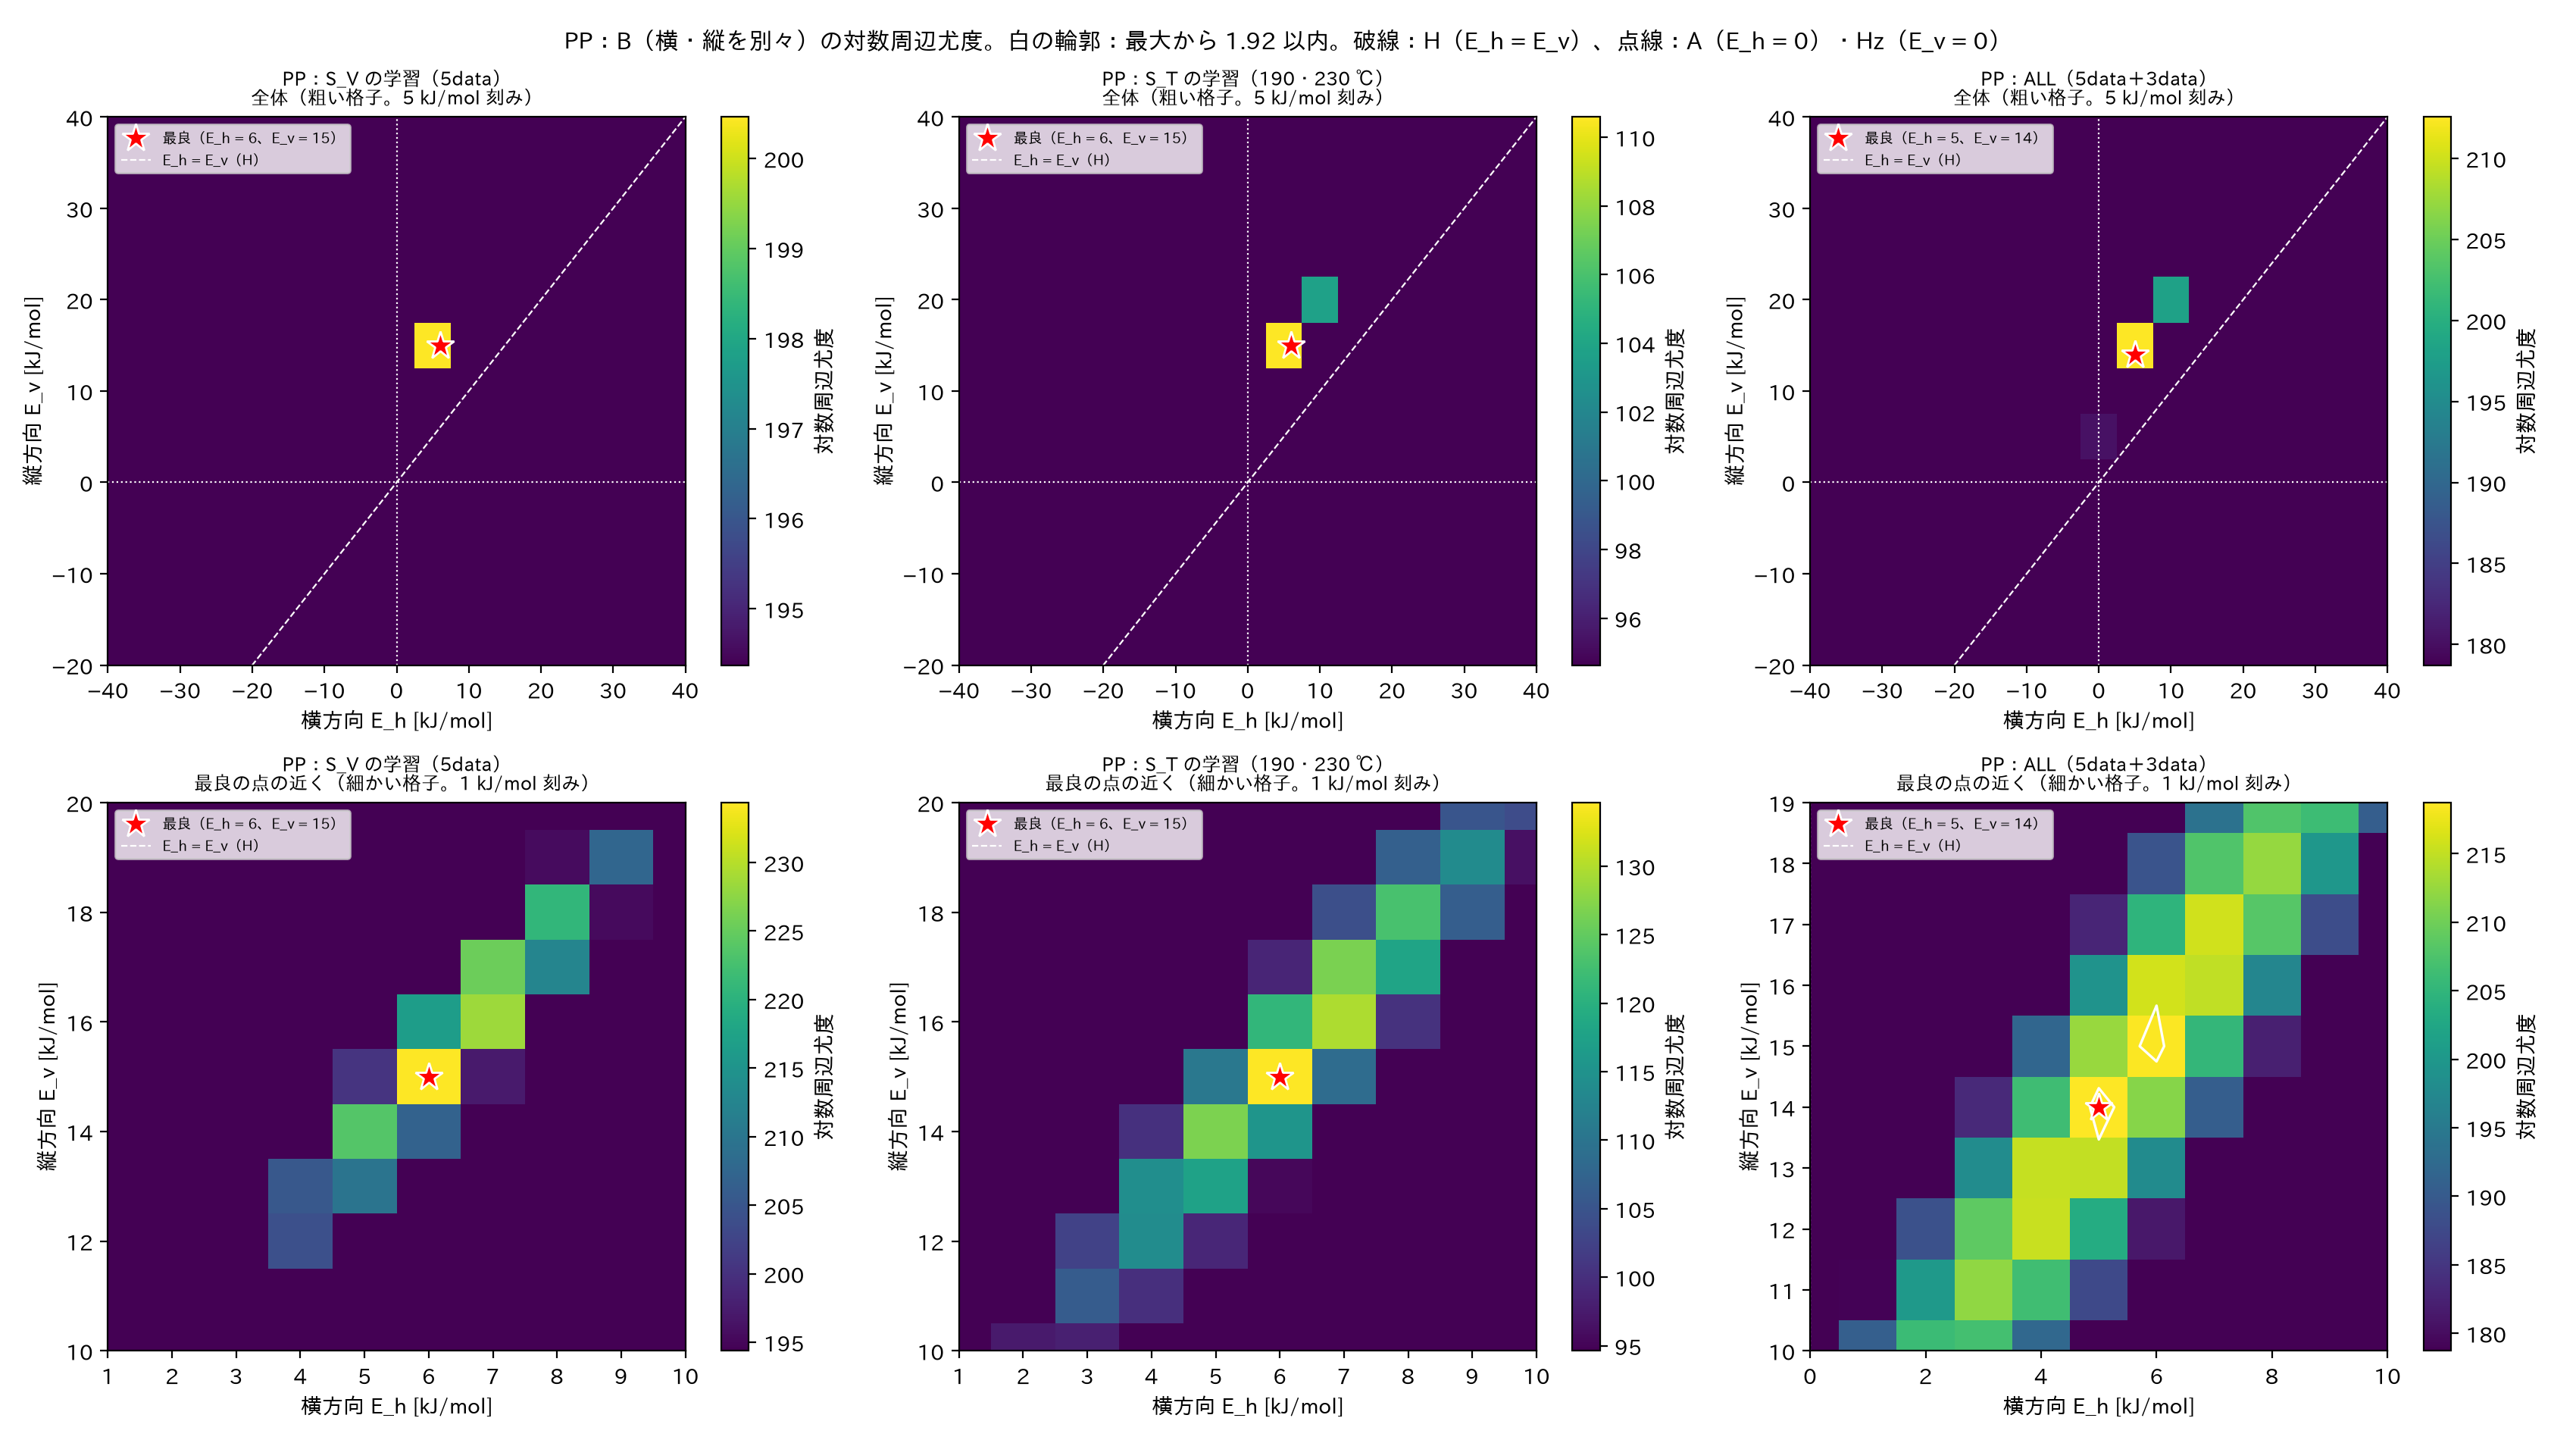
\includegraphics[width=\linewidth]{fig2a_profile_2d_B_PP.png}
\caption{PP：$\Eh$ と $\Ev$ を振ったときの LML（上段：全体、下段：最良の点の近く）}
\end{figure}
\begin{points}
\pt{ファイル}\file{results/step5a/fig2a_profile_2d_B_PP.png}（PP）、\file{fig2b_profile_2d_B_MIX.png}（粉砕材混合 PP）
\pt{何を示す図か}B では、横方向のずれ $\Eh$ と縦方向のずれ $\Ev$ を別々に決めます。2 つの $E$ の組ごとの LML を、色で描いた図です（黄色いほど良い）。
\pt{軸と記号}横軸が $\Eh$、縦軸が $\Ev$ [kJ/mol]。上段は粗い格子（5 kJ/mol 刻み）、下段は最良の点の近くの細かい格子（1 kJ/mol 刻み）。赤い星が最良の点、白い破線が $\Eh=\Ev$（H の構造）、白い点線の縦線が $\Eh=0$（A の構造）、横線が $\Ev=0$（Hz の構造）です。下段の白い輪郭は、最大から 1.92 以内の範囲です。
\pt{見るポイント}黄色い領域が、破線（H）の上にあるか、縦の点線（A）の近くにあるか。領域がどんな形（細長い斜めの帯なら、2 つの $E$ の組み合わせが決まりきらない）か。
\pt{今回の結果}最良の点は、PP で $(\Eh,\Ev) = $ (6, 15)、粉砕材混合 PP で (6, 15) kJ/mol（S\_V の学習）で、破線（H）からはずっと離れた、$\Eh$ が小さく $\Ev$ が大きい側にあります。LML は A より 78・54 大きくなります。ただし、下段のように、高い領域は斜めの細長い帯になっていて、$\Eh$ と $\Ev$ を別々には決めきれません。帯に沿った方向には、LML がゆるやかにしか変わらず、帯に垂直な方向（差 $\Ev-\Eh$ が約 9 kJ/mol からずれる方向）には、急に下がります。つまり、「$\Ev-\Eh$ ≈ 9 kJ/mol」という組み合わせが、データで決まっています。
\end{points}

\subsection{図3：マスターカーブ}
\begin{figure}[H]
\centering
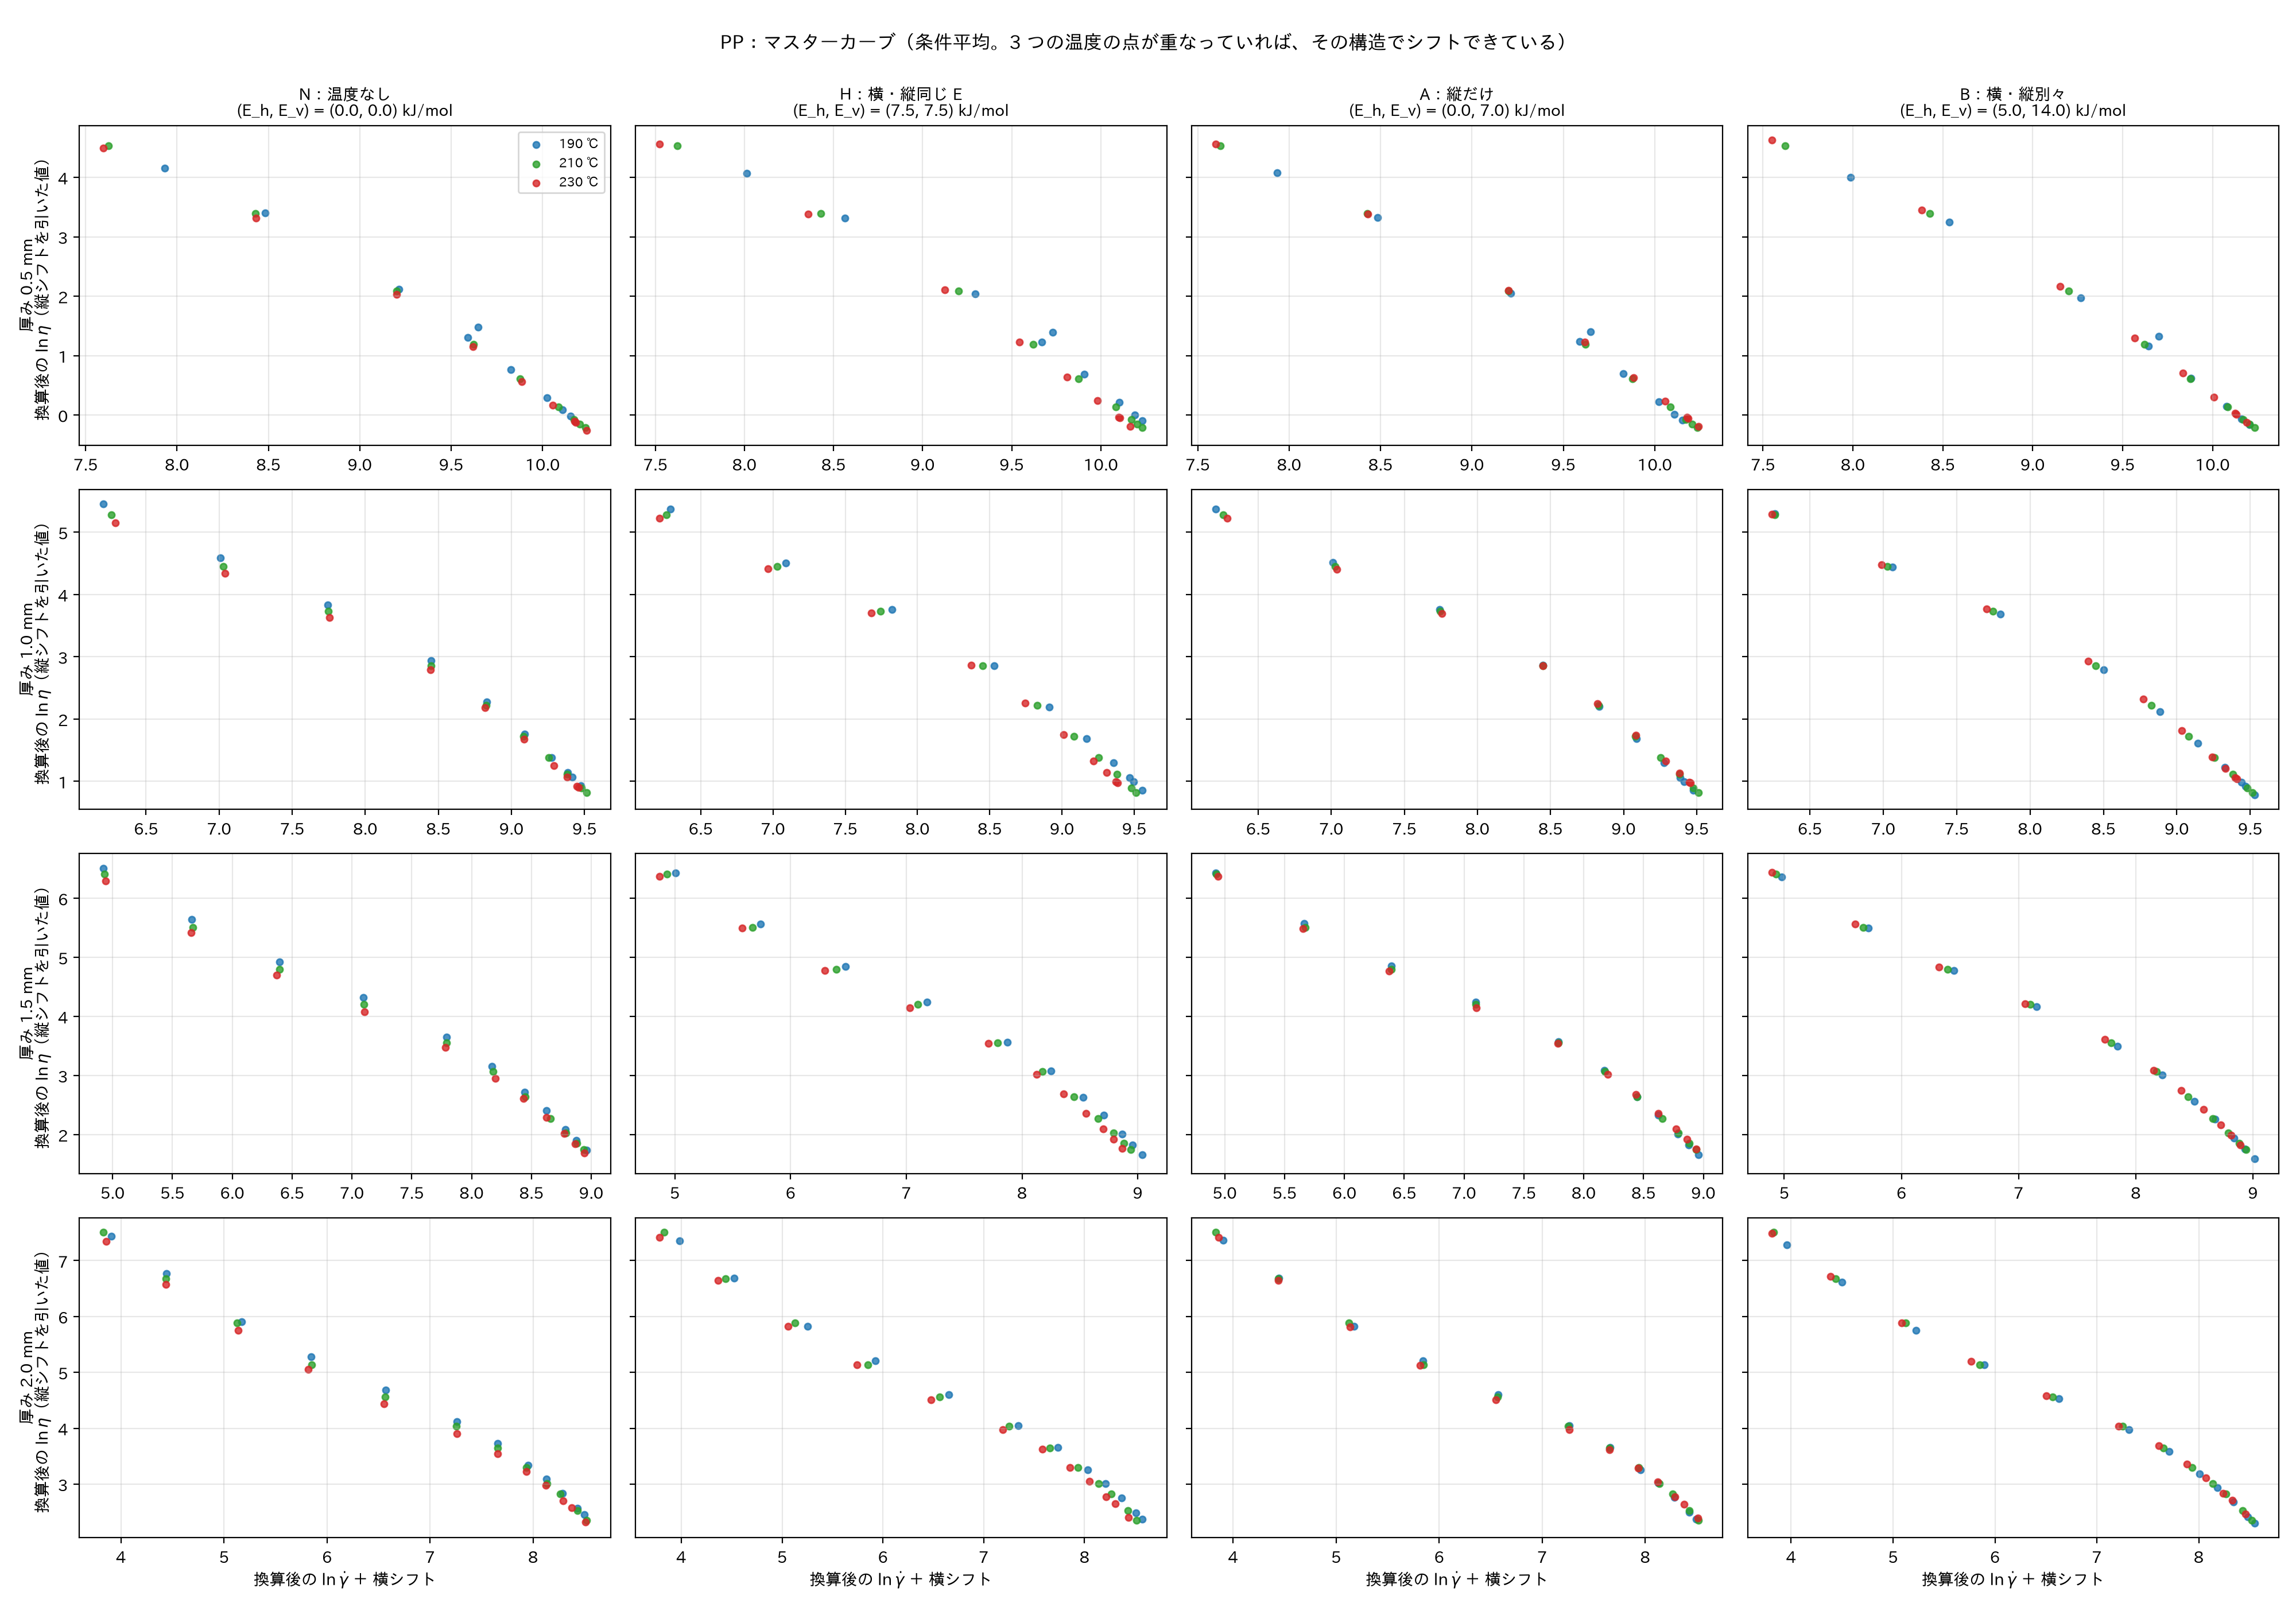
\includegraphics[width=0.95\linewidth]{fig3a_master_curve_PP.png}
\caption{PP：換算後の条件平均のデータ（色：設定温度。列：構造、行：厚み）}
\end{figure}
\begin{points}
\pt{ファイル}\file{results/step5a/fig3a_master_curve_PP.png}（PP）、\file{fig3b_master_curve_MIX.png}（粉砕材混合 PP）
\pt{何を示す図か}構造ごとに、最良の $E$ でデータを換算（シフト）して重ねた図です。「その構造で、3 つの温度のデータが 1 本の曲線に重なるか」を、目で確かめます。
\pt{軸と記号}横軸が、横シフト後の $\ln\gd$、縦軸が、縦シフトを引いた後の $\ln\eta$。青 190 ℃、緑 210 ℃、赤 230 ℃。行が厚み、列が構造（N：温度なし、H、A、B）です。
\pt{見るポイント}同じ色の点が離れて、温度ごとの帯に分かれていないか。青・緑・赤が重なっていれば、よく換算できています。
\pt{今回の結果}N（温度なし）は、同じ位置で、青・緑・赤が縦にずれています（190 ℃ が上）。A と B では、3 つの色がほぼ重なります。H は、横にずらすことで、かえって点が散らばります（特に低せん断速度側）。
\end{points}

\subsection{図4：設定温度ごとの予測曲線}
\begin{figure}[H]
\centering
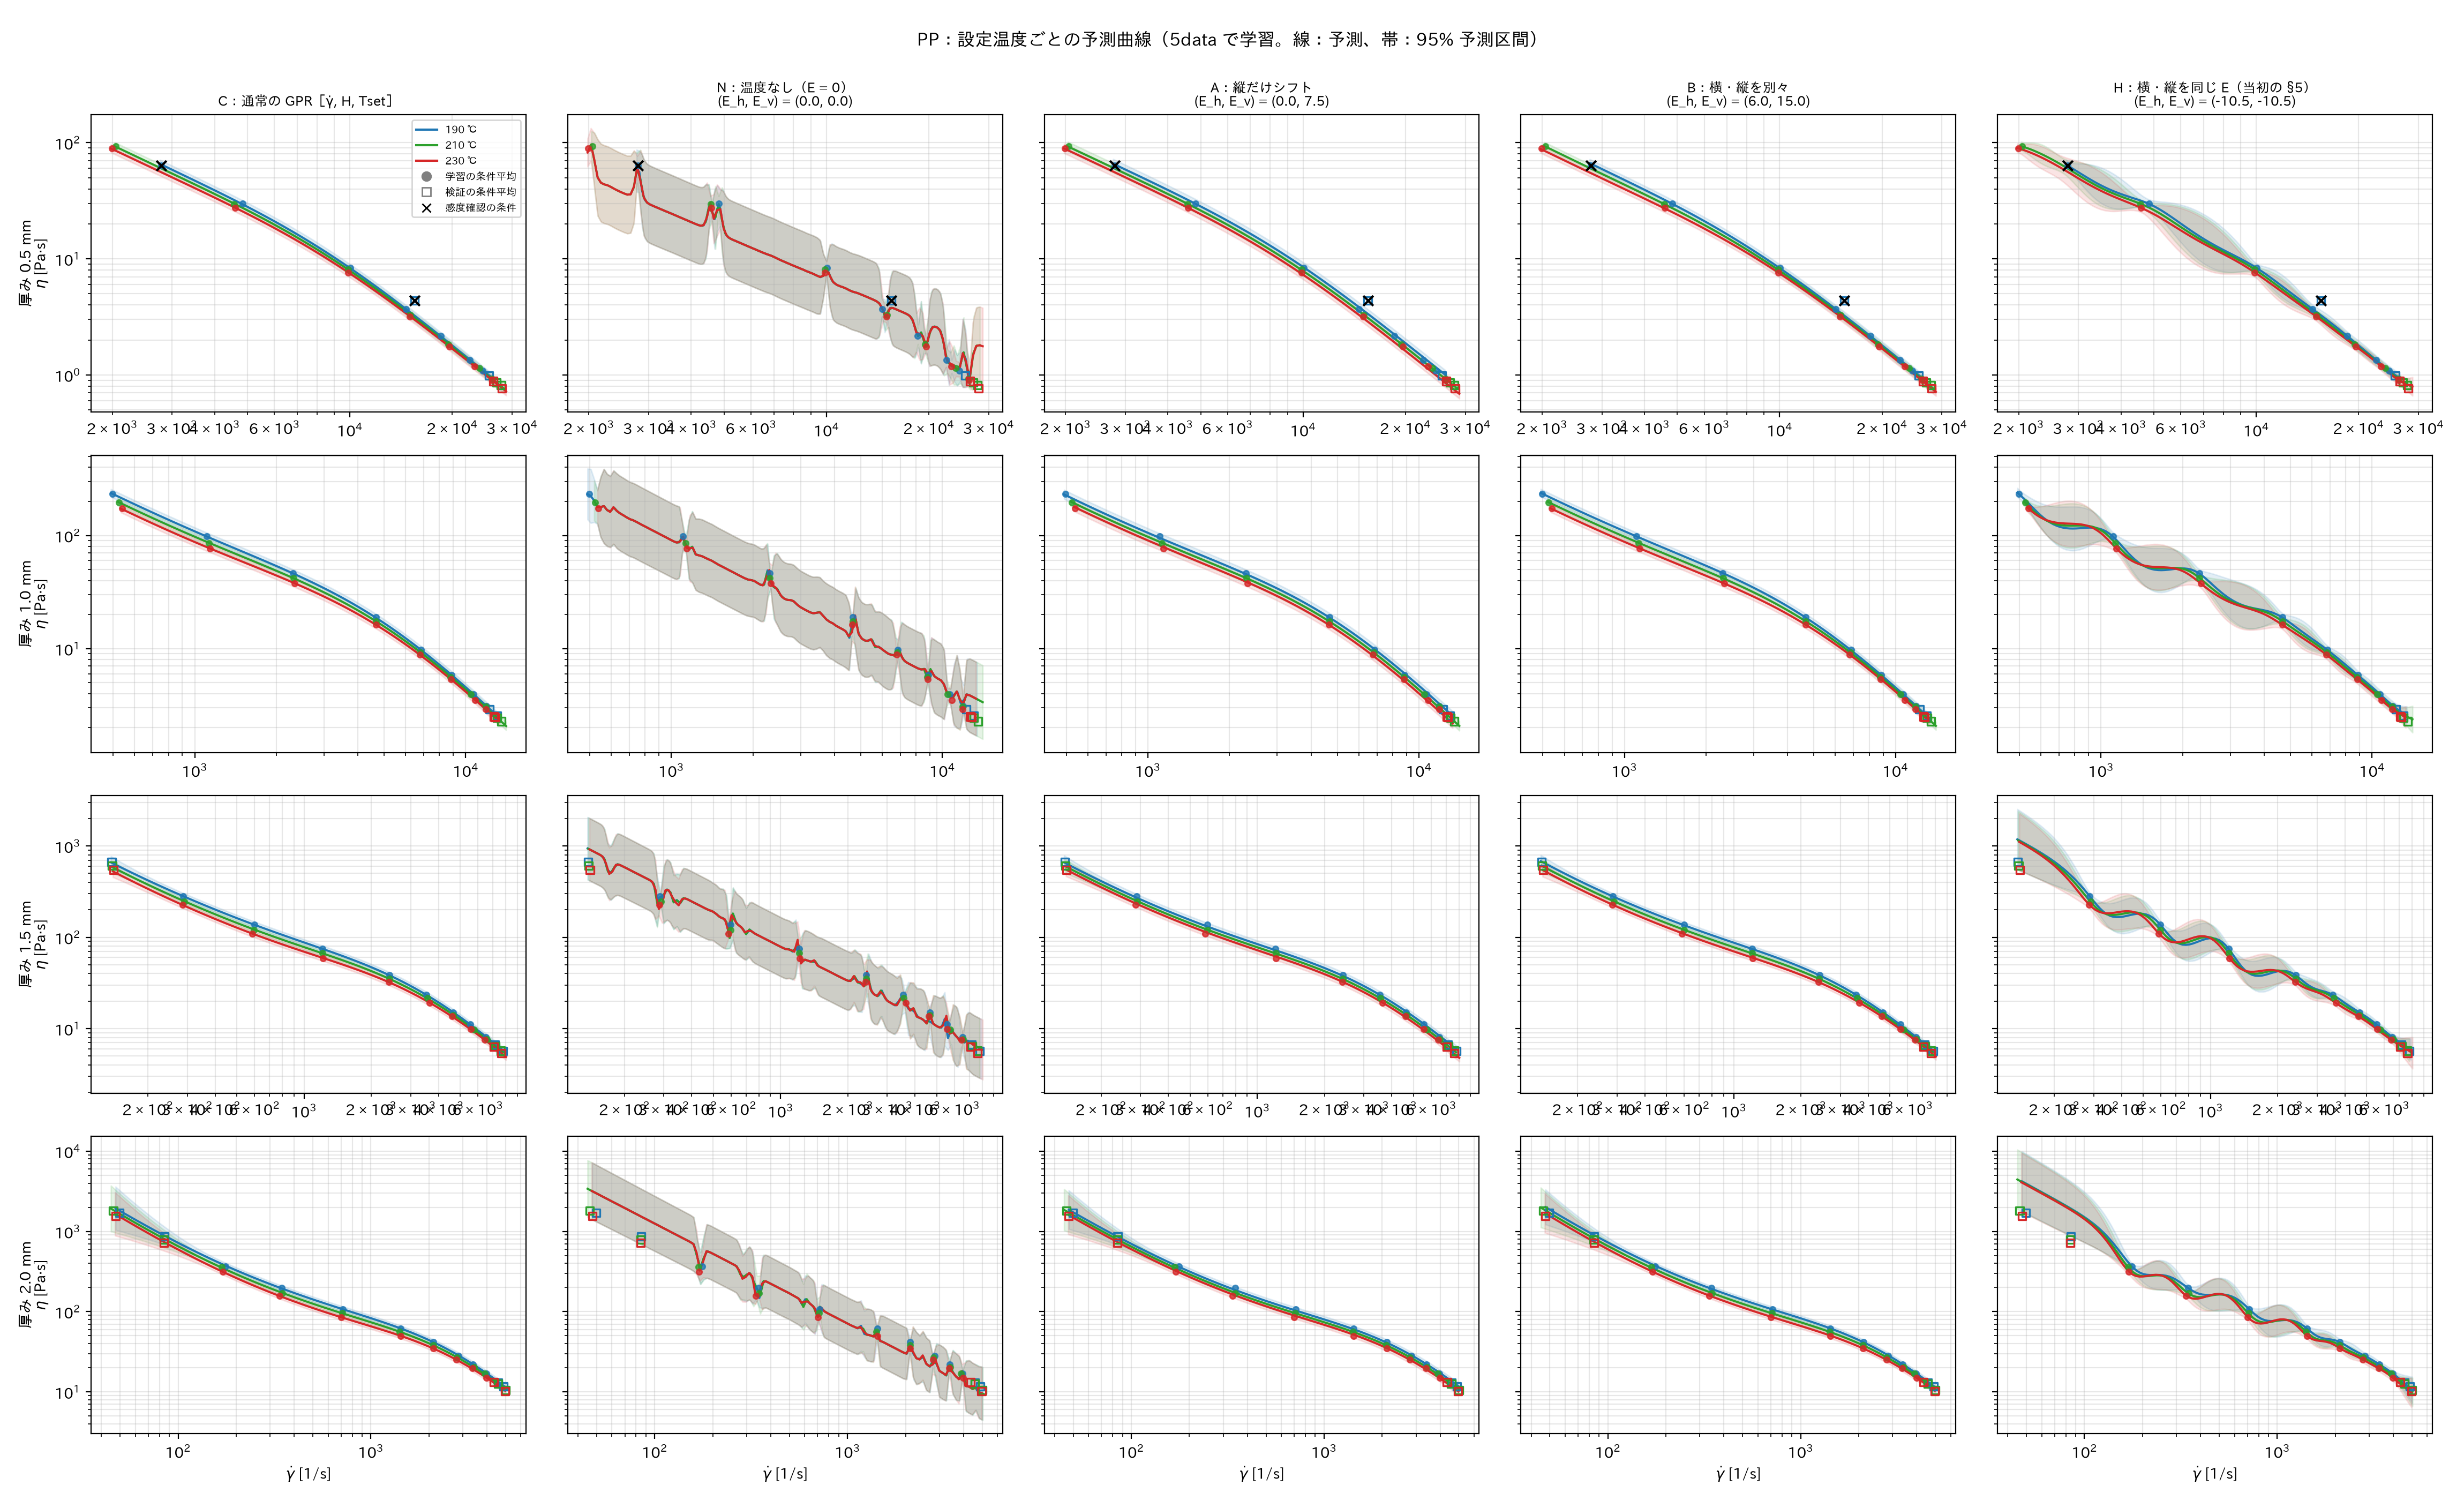
\includegraphics[width=\linewidth]{fig4a_curves_PP.png}
\caption{PP：設定温度ごとの予測曲線（5data で学習。列：構造、行：厚み）}
\end{figure}
\begin{points}
\pt{ファイル}\file{results/step5a/fig4a_curves_PP.png}（PP）、\file{fig4b_curves_MIX.png}（粉砕材混合 PP）
\pt{何を示す図か}5data で学習したモデルの、設定温度ごとの予測曲線と 95\% 予測区間を、データと重ねた図です。
\pt{軸と記号}横軸が $\gd$、縦軸が $\eta$（どちらも対数軸）。線の色が設定温度、帯が予測区間。塗りつぶしの丸が学習の条件平均、白抜きの四角が検証（3data）の条件平均、黒い×が感度確認の条件です。列は、C（通常の GPR）、N、A、B、H。
\pt{見るポイント}(1) 3 本の線が、温度の順（190 ℃ が上）に並ぶか。(2) 白抜きの四角（外挿の検証データ）が、線と帯の上に乗るか。(3) 帯が、学習範囲の外で広がるか。(4) 線がなめらかか。
\pt{今回の結果}C・A・B は、3 本の線が順に並び、外挿の四角（低速側・高速側）にも乗ります。A は、温度間の比が一定（縦シフトのみ）です。N は、帯が広く、線がでこぼこです（温度が分からないため）。H は、線が波打ち、学習範囲の端で帯が大きく広がります。
\end{points}

\subsection{図5：評価指標の比較}
\begin{figure}[H]
\centering
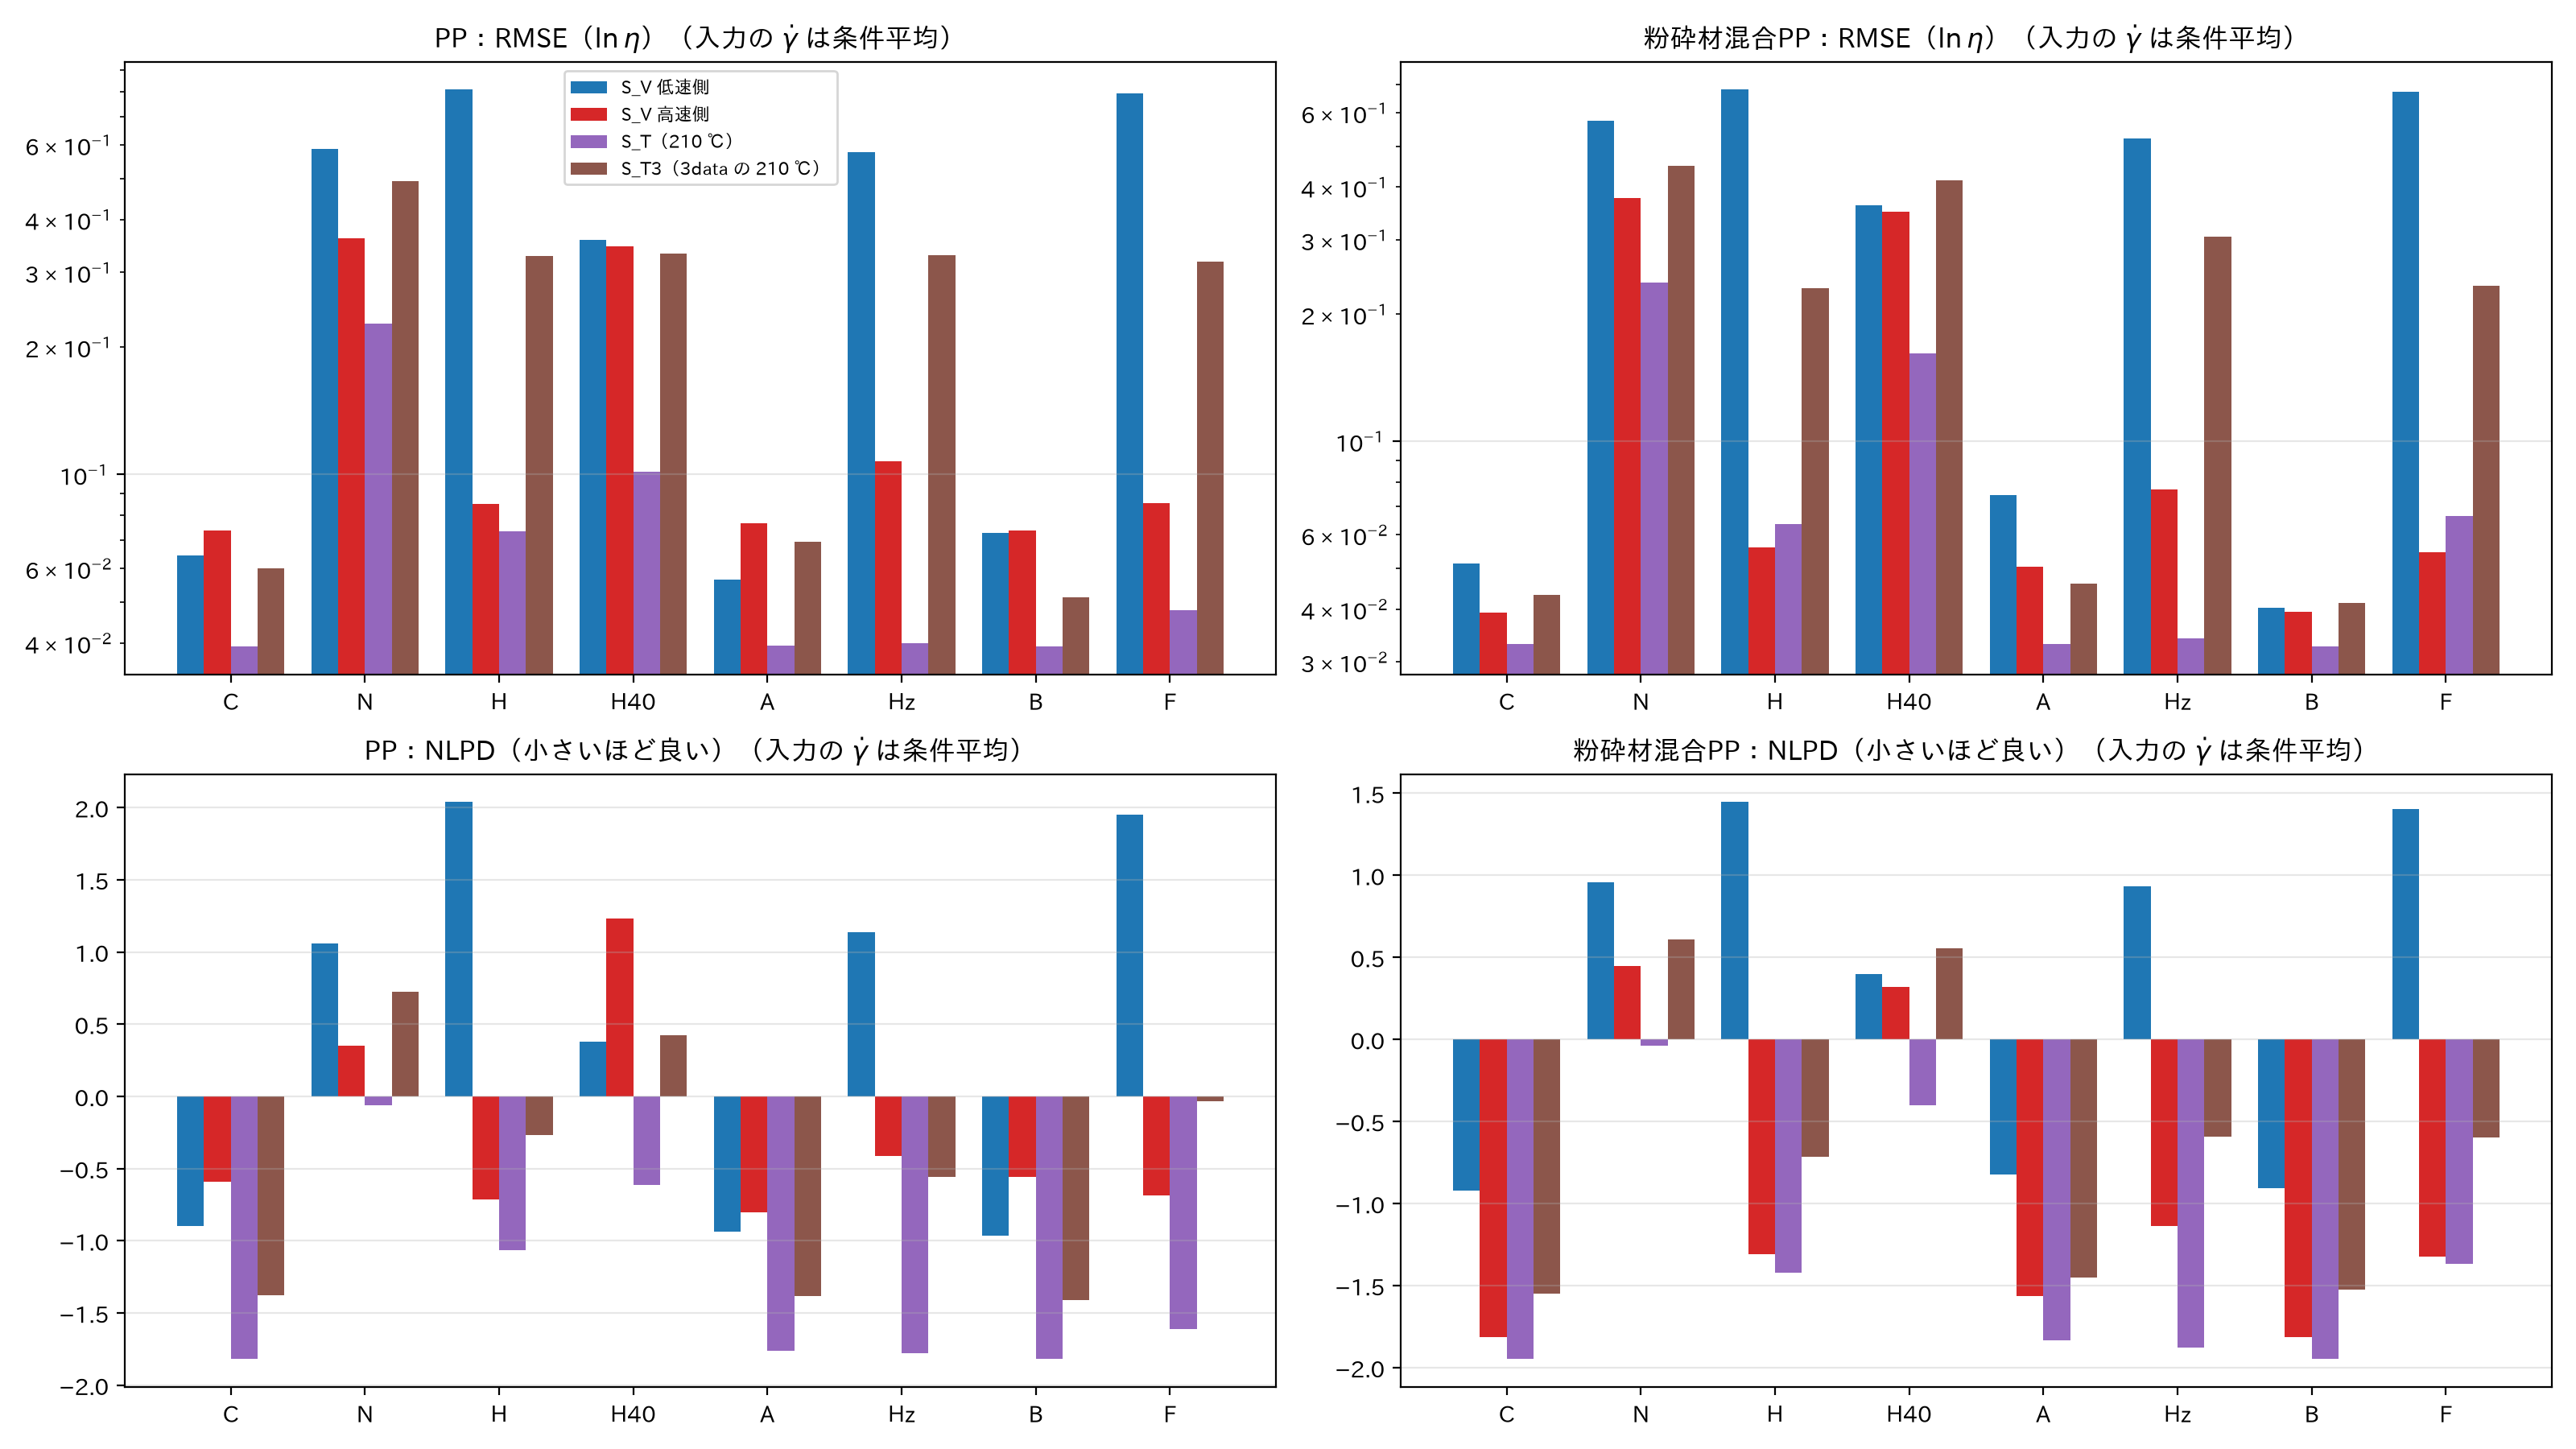
\includegraphics[width=0.95\linewidth]{fig5_metrics.png}
\caption{構造ごとの RMSE（上段）と NLPD（下段）}
\end{figure}
\begin{points}
\pt{ファイル}\file{results/step5a/fig5_metrics.png}
\pt{何を示す図か}構造ごとの予測精度を、検証データの種類ごとに比べた図です。入力の $\gd$ は条件平均です。
\pt{軸と記号}横軸が構造、縦軸が RMSE（上段。対数軸）と NLPD（下段。小さいほど良い）。棒の色が検証データ：青 S\_V 低速側、赤 S\_V 高速側、紫 S\_T（210 ℃）、茶 S\_T3（3data の 210 ℃）。
\pt{見るポイント}C を基準にして、A・B が同等以上か（棒が同じか低いか）。N・H・H40・Hz・F が、どこで悪いか。
\pt{今回の結果}A と B は、C とほぼ同じ高さです（表\ref{tab:m_pp}・\ref{tab:m_mix}）。N は、どの検証でも大きく外れ、H・H40・F は、低速側と S\_T3 で大きく外れます。
\end{points}

\subsection{図6：設定温度の効果}
\begin{figure}[H]
\centering
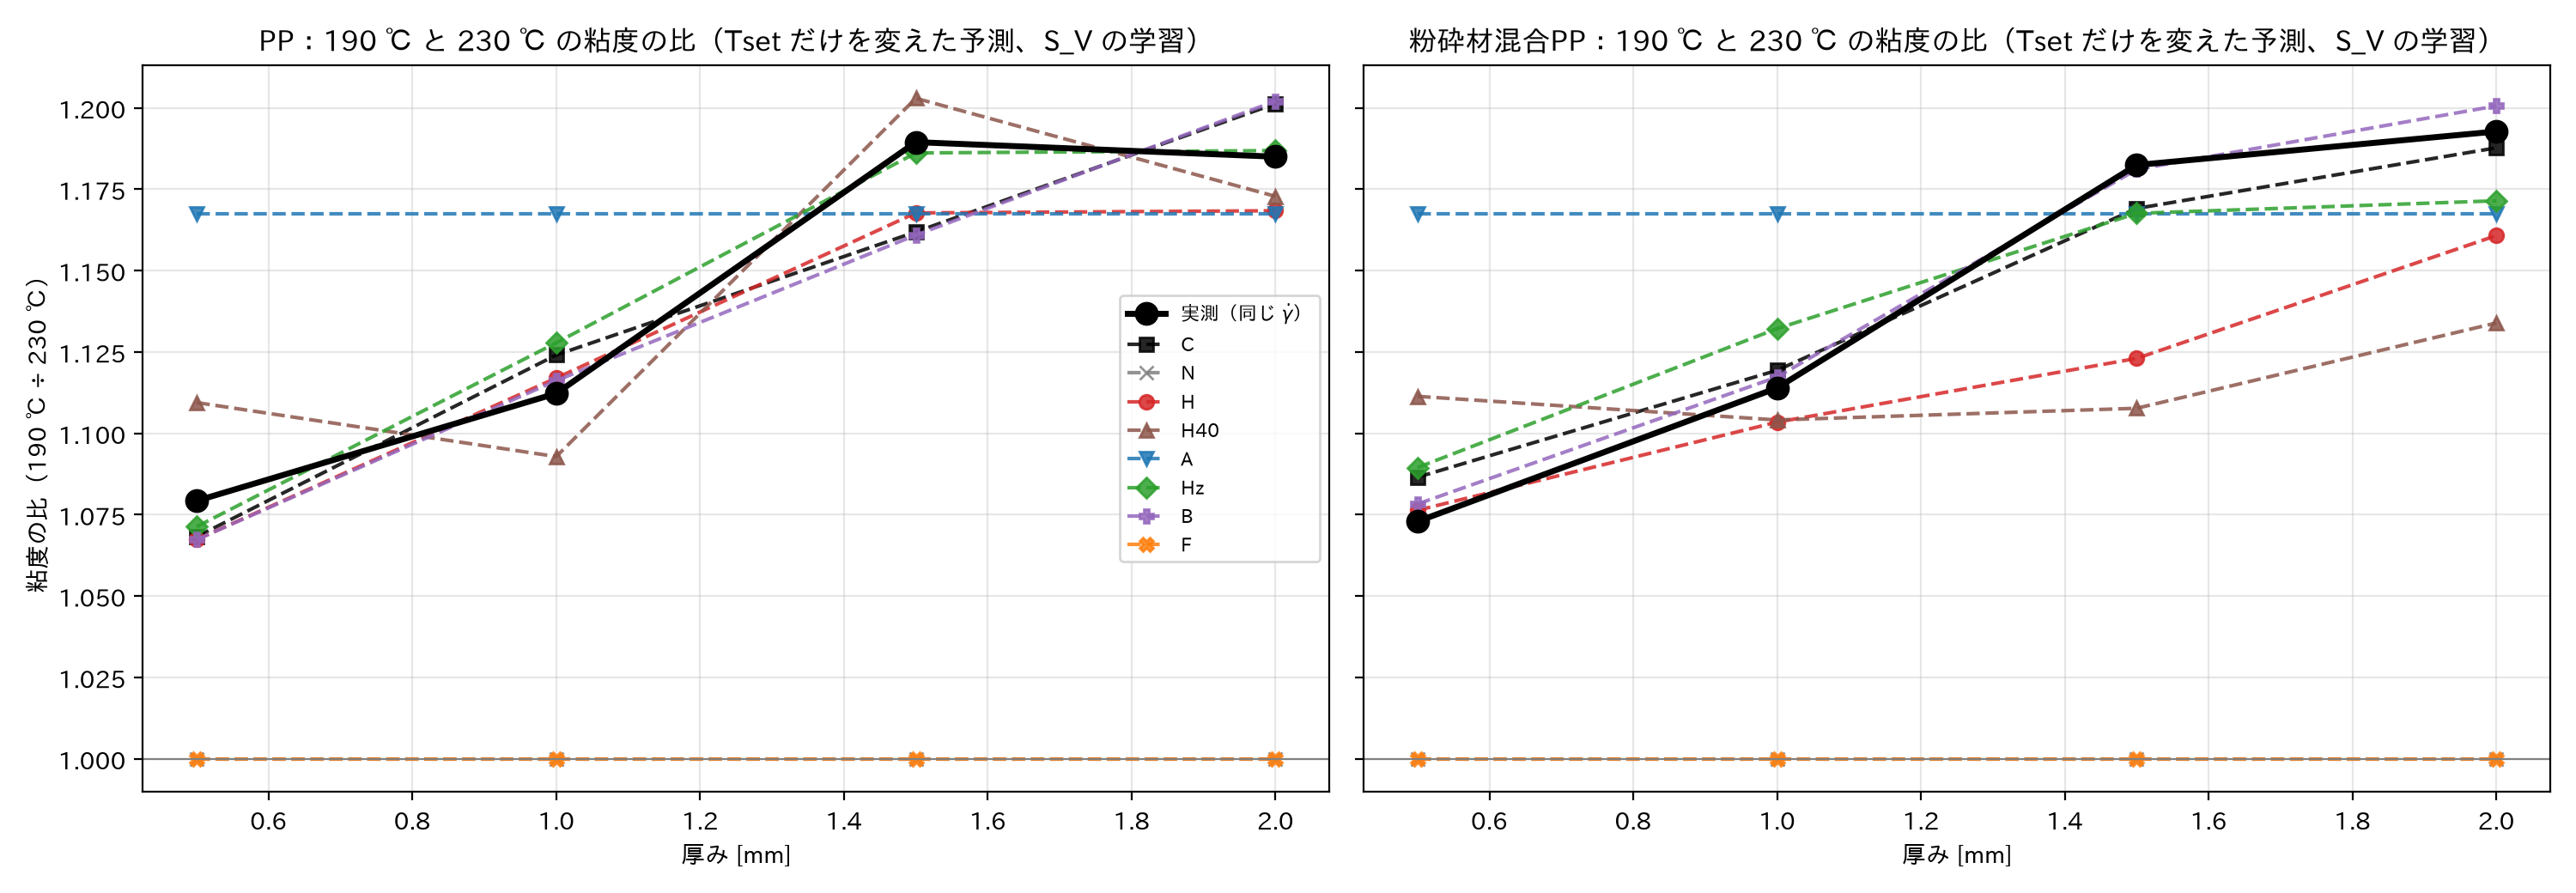
\includegraphics[width=\linewidth]{fig6_temperature_effect.png}
\caption{190 ℃ と 230 ℃ の粘度の比（Tset だけを変えた予測）。黒の太線が実測}
\end{figure}
\begin{points}
\pt{ファイル}\file{results/step5a/fig6_temperature_effect.png}
\pt{何を示す図か}同じ厚み・同じせん断速度で、190 ℃ の粘度が 230 ℃ の何倍かを、実測と各構造の予測で比べた図です。
\pt{軸と記号}横軸が厚み、縦軸が粘度の比（190 ℃ ÷ 230 ℃）。黒の太線が実測、色の破線が構造ごとの予測です。比が 1 なら、温度の効果なし。
\pt{見るポイント}実測の線（右上がり：厚いほど効果が大きい）に、予測が近いか。A のように、水平な線（厚みによらず一定）になっていないか。
\pt{今回の結果}実測の比は、厚み 0.5 mm で約 1.08、2.0 mm で約 1.19 と、厚いほど大きくなります。A は一定の比（1.17）で、この厚み依存を表せません。C と B は、厚み依存を表せています（表\ref{tab:eff}）。
\end{points}

\subsection{高解像度のグラフ（報告書・発表資料用）}
\begin{points}
\pt{ファイル}\file{results/step5a/highres/hr_<材料>_<構造>_<学習>_by-thickness_<厚み>mm.png}（厚みごとに 1 枚。3 つの設定温度の曲線）と、\file{..._by-temperature_<温度>C.png}（設定温度ごとに 1 枚。4 つの厚みの曲線）。Git には入れません（ノートのセルで、いつでも作り直せます）。
\pt{何を示す図か}GPR6月のノートのセル9-2 と同じ見せ方の、せん断速度 ― 粘度の学習結果グラフです。\textbf{600 dpi（15 $\times$ 10 インチ）}で、1 枚に 1 つのグラフを保存します。線は予測の平均、帯は 95\% 予測区間、塗りつぶしの点は学習に使った条件（条件平均）、白抜きの点は学習に使わなかった条件（検証）、黒い $\times$ は問題データ一覧の「感度確認」の条件です。既定では、本命 B と対案 A を、PP と粉砕材混合 PP について描きます。
\pt{変え方}ノート末尾の「高解像度のグラフ」のセルの先頭に、設定エリアがあります（描く構造・材料・学習の種類、レイアウト、帯、点、軸の範囲、予測線の延長、図の大きさ・解像度、文字・点・線の大きさ、タイトルと軸名の表示、保存形式 png・pdf・svg）。\textbf{そのセルの設定だけを直して、そのセルだけを実行し直せます}（学習はやり直しません。ノート全体を一度実行した後で）。
\pt{見るポイント}(1) 設定温度ごとの線が、温度の順に並ぶか。(2) 白抜きの点（外挿の検証データ）が、線と帯の上に乗るか。(3) 帯が、学習範囲の外で広がるか。
\end{points}

% =====================================================================
\section{表の見方}

\begin{table}[H]
\caption{最良の $E$ と対数周辺尤度（\file{best_E.csv}）。$E$ の範囲：LML が最大から 1.92 以内。差：温度なし（$E=0$）との LML の差}\label{tab:best}
\begin{tabularx}{\linewidth}{@{}l>{\raggedright\arraybackslash}p{4.5\zw}l>{\raggedright\arraybackslash}p{9\zw}rr@{}}
\toprule
材料 & 学習 & 構造 & 最良の $E$ [kJ/mol]（範囲） & LML & 差 \\
\midrule
PP & S\_V の学習 & H & $-$10.5（$-$13.5〜$-$10.5） & 88.4 & 5.5 \\
 &  & A & 7.5（7.0〜8.0） & 156.3 & 73.5 \\
 &  & Hz & $-$7.0（$-$7.5〜$-$6.0） & 120.3 & 37.5 \\
 &  & B & ($\Eh$, $\Ev$) = (6, 15) & 234.4 & 151.5 \\
 &  & F & $-$11.0（$-$15.0〜$-$10.0） & 90.0 & 7.1 \\
 & S\_T の学習 & H & $-$3.0（$-$5.0〜0.0） & 36.9 & 0.9 \\
 &  & A & 7.5（6.5〜8.0） & 82.5 & 46.6 \\
 &  & Hz & $-$4.5（$-$5.5〜$-$3.5） & 57.0 & 21.0 \\
 &  & B & ($\Eh$, $\Ev$) = (6, 15) & 134.6 & 98.7 \\
 &  & F & $-$3.0（$-$7.5〜0.0） & 36.6 & 0.6 \\
 & ALL & H & 7.5（7.0〜9.5） & 124.5 & 7.3 \\
 &  & A & 7.0（6.5〜7.5） & 191.9 & 74.6 \\
 &  & Hz & $-$4.0（$-$4.5〜$-$3.5） & 156.7 & 39.5 \\
 &  & B & ($\Eh$, $\Ev$) = (5, 14) & 218.7 & 101.5 \\
 &  & F & $-$4.5（$-$7.5〜7.5） & 120.5 & 3.3 \\
粉砕材混合 PP & S\_V の学習 & H & $-$10.0（$-$12.5〜$-$7.5） & 93.2 & 10.7 \\
 &  & A & 7.5（7.0〜8.0） & 152.1 & 69.5 \\
 &  & Hz & $-$6.5（$-$7.5〜$-$6.0） & 125.9 & 43.4 \\
 &  & B & ($\Eh$, $\Ev$) = (6, 15) & 206.2 & 123.7 \\
 &  & F & $-$10.5（$-$15.0〜$-$7.5） & 97.8 & 15.3 \\
 & S\_T の学習 & H & $-$3.5（$-$7.5〜0.0） & 36.9 & 1.2 \\
 &  & A & 7.5（6.5〜8.0） & 79.7 & 43.9 \\
 &  & Hz & $-$4.5（$-$5.5〜$-$3.5） & 56.8 & 21.0 \\
 &  & B & ($\Eh$, $\Ev$) = (6, 15) & 113.9 & 78.1 \\
 &  & F & $-$3.5（$-$7.5〜0.0） & 36.6 & 0.8 \\
 & ALL & H & $-$8.5（$-$11.5〜$-$7.5） & 160.8 & 31.5 \\
 &  & A & 7.0（6.5〜7.0） & 220.5 & 91.2 \\
 &  & Hz & $-$6.5（$-$6.5〜$-$6.0） & 197.7 & 68.5 \\
 &  & B & ($\Eh$, $\Ev$) = (6, 15) & 303.6 & 174.4 \\
 &  & F & $-$10.5（$-$12.5〜$-$7.5） & 166.4 & 37.2 \\
\bottomrule
\end{tabularx}
\end{table}

\begin{table}[H]
\caption{検証の指標：PP（入力の $\gd$ は条件平均。\file{metrics.csv}）。RMSE と NLPD}\label{tab:m_pp}
\begin{tabularx}{\linewidth}{@{}l*{8}{r}@{}}
\toprule
 & \multicolumn{4}{c}{RMSE} & \multicolumn{4}{c}{NLPD} \\
\cmidrule(lr){2-5}\cmidrule(l){6-9}
構造 & S\_V 低 & S\_V 高 & S\_T & S\_T3 & S\_V 低 & S\_V 高 & S\_T & S\_T3 \\
\midrule
C & 0.064 & 0.074 & 0.039 & 0.060 & $-0.90$ & $-0.59$ & $-1.82$ & $-1.38$ \\
N & 0.588 & 0.361 & 0.227 & 0.493 & 1.06 & 0.35 & $-0.06$ & 0.73 \\
H & 0.810 & 0.085 & 0.073 & 0.327 & 2.04 & $-0.72$ & $-1.07$ & $-0.27$ \\
H40 & 0.358 & 0.346 & 0.101 & 0.332 & 0.38 & 1.23 & $-0.61$ & 0.42 \\
A & 0.057 & 0.077 & 0.040 & 0.069 & $-0.94$ & $-0.80$ & $-1.76$ & $-1.38$ \\
Hz & 0.578 & 0.107 & 0.040 & 0.330 & 1.13 & $-0.41$ & $-1.78$ & $-0.56$ \\
B & 0.073 & 0.074 & 0.039 & 0.051 & $-0.96$ & $-0.56$ & $-1.82$ & $-1.41$ \\
F & 0.793 & 0.086 & 0.048 & 0.319 & 1.95 & $-0.69$ & $-1.61$ & $-0.03$ \\
\bottomrule
\end{tabularx}
\end{table}

\begin{table}[H]
\caption{検証の指標：粉砕材混合 PP（入力の $\gd$ は条件平均）}\label{tab:m_mix}
\begin{tabularx}{\linewidth}{@{}l*{8}{r}@{}}
\toprule
 & \multicolumn{4}{c}{RMSE} & \multicolumn{4}{c}{NLPD} \\
\cmidrule(lr){2-5}\cmidrule(l){6-9}
構造 & S\_V 低 & S\_V 高 & S\_T & S\_T3 & S\_V 低 & S\_V 高 & S\_T & S\_T3 \\
\midrule
C & 0.051 & 0.039 & 0.033 & 0.043 & $-0.92$ & $-1.82$ & $-1.95$ & $-1.55$ \\
N & 0.574 & 0.376 & 0.238 & 0.450 & 0.96 & 0.45 & $-0.04$ & 0.61 \\
H & 0.681 & 0.056 & 0.064 & 0.231 & 1.45 & $-1.31$ & $-1.42$ & $-0.72$ \\
H40 & 0.362 & 0.350 & 0.161 & 0.415 & 0.40 & 0.32 & $-0.40$ & 0.56 \\
A & 0.074 & 0.050 & 0.033 & 0.046 & $-0.82$ & $-1.56$ & $-1.84$ & $-1.45$ \\
Hz & 0.521 & 0.077 & 0.034 & 0.305 & 0.93 & $-1.14$ & $-1.88$ & $-0.59$ \\
B & 0.040 & 0.039 & 0.033 & 0.041 & $-0.91$ & $-1.81$ & $-1.95$ & $-1.52$ \\
F & 0.673 & 0.054 & 0.066 & 0.234 & 1.41 & $-1.33$ & $-1.37$ & $-0.60$ \\
\bottomrule
\end{tabularx}
\end{table}

\begin{table}[H]
\caption{本命（B）と対案（A）の比較（\file{main_vs_alt.csv}。基準は C）。LML と RMSE は S\_V の学習、差は温度なし（$E=0$）との LML の差、($\Eh$, $\Ev$) は ALL の学習での最良の値（kJ/mol）。RMSE の入力の $\gd$ は条件平均。構造の「---」は、$E$ をもたない構造}\label{tab:main}
{\small
\setlength{\tabcolsep}{3.2pt}
\begin{tabular}{@{}llcrrrrrrr@{}}
\toprule
材料 & 役割 & 構造 & ($\Eh$, $\Ev$) & LML & 差 & \multicolumn{4}{c}{RMSE（$\ln\eta$）} \\
\cmidrule(l){7-10}
 & & & & & & S\_V 低 & S\_V 高 & S\_T & S\_T3 \\
\midrule
PP & 本命 & B & (5.0, 14.0) & 234.4 & 151.5 & 0.073 & 0.074 & 0.039 & 0.051 \\
 & 対案 & A & (0.0, 7.0) & 156.3 & 73.5 & 0.057 & 0.077 & 0.040 & 0.069 \\
 & 基準 & C & --- & --- & --- & 0.064 & 0.074 & 0.039 & 0.060 \\
粉砕材混合 PP & 本命 & B & (6.0, 15.0) & 206.2 & 123.7 & 0.040 & 0.039 & 0.033 & 0.041 \\
 & 対案 & A & (0.0, 7.0) & 152.1 & 69.5 & 0.074 & 0.050 & 0.033 & 0.046 \\
 & 基準 & C & --- & --- & --- & 0.051 & 0.039 & 0.033 & 0.043 \\
\bottomrule
\end{tabular}}
\end{table}

\begin{table}[H]
\caption{190 ℃ と 230 ℃ の粘度の比（S\_V の学習。\file{tset_effect.csv}、\file{observed_ratio.csv}）}\label{tab:eff}
\begin{tabularx}{\linewidth}{@{}l>{\raggedright\arraybackslash}p{5\zw}rrrr@{}}
\toprule
材料 & 構造 & 0.5 mm & 1.0 mm & 1.5 mm & 2.0 mm \\
\midrule
PP & 実測 & 1.079 & 1.112 & 1.189 & 1.185 \\
 & C & 1.068 & 1.124 & 1.162 & 1.201 \\
 & A & 1.167 & 1.167 & 1.167 & 1.167 \\
 & Hz & 1.071 & 1.128 & 1.186 & 1.187 \\
 & B & 1.067 & 1.116 & 1.161 & 1.202 \\
 & H & 1.067 & 1.117 & 1.168 & 1.168 \\
 & H40 & 1.109 & 1.093 & 1.203 & 1.173 \\
粉砕材混合 PP & 実測 & 1.073 & 1.114 & 1.182 & 1.193 \\
 & C & 1.087 & 1.119 & 1.169 & 1.188 \\
 & A & 1.167 & 1.167 & 1.167 & 1.167 \\
 & Hz & 1.089 & 1.132 & 1.168 & 1.171 \\
 & B & 1.078 & 1.117 & 1.181 & 1.201 \\
 & H & 1.076 & 1.103 & 1.123 & 1.161 \\
 & H40 & 1.111 & 1.104 & 1.108 & 1.134 \\
\bottomrule
\end{tabularx}
\end{table}

\begin{table}[H]
\caption{感度確認：P02（190 ℃・0.5 mm・20 mm/s）を除いた場合の、最良の $E$（S\_V の学習。\file{sensitivity_E.csv}）}\label{tab:sens}
\begin{tabularx}{\linewidth}{@{}l>{\raggedright\arraybackslash}p{4\zw}rrr@{}}
\toprule
材料 & 構造 & すべて & P02 を除く & 動き \\
\midrule
 & A & 7.5 & 7.5 & 0.0 \\
粉砕材混合 PP & H & $-$10.0 & $-$10.0 & 0.0 \\
 & A & 7.5 & 7.5 & 0.0 \\
PP & H & $-$10.5 & $-$10.0 & 0.5 \\
\bottomrule
\end{tabularx}
\end{table}

\begin{table}[H]
\caption{\file{results/step5a/} の表}
\begin{tabularx}{\linewidth}{@{}>{\raggedright\arraybackslash}p{19\zw}X@{}}
\toprule
ファイル & 中身と主な列 \\
\midrule
\file{profile_likelihood.csv} & プロファイルの全点。\file{set}（S\_V・S\_T・ALL）、\file{structure}（H・A・Hz・B・F）、\file{E}（1 次元）、\file{Eh}・\file{Ev}、\file{LML}、\file{noise_sd}、\file{stage}（粗い格子・細かい格子）。 \\
\file{best_E.csv} & 構造ごとの最良の $E$（B は \file{Eh_best}・\file{Ev_best}）、\file{LML_best}、\file{dLML_vs_E0}（温度なしとの差）、\file{E_95_lo}・\file{E_95_hi}（1.92 以内の範囲）、\file{LML_at_E40}。 \\
\file{metrics.csv} & 構造（\file{variant}）・入力の $\gd$（\file{mode}：cm・shot）・検証の種類（\file{split}）・範囲（\file{subset}）ごとの指標。 \\
\file{kernels.csv} & 評価用に学習した GPR のハイパーパラメータ（\file{Eh}・\file{Ev}、\file{LML}、\file{noise_sd}、下限への張り付き）。 \\
\file{tset_effect.csv} & 設定温度の効果（Tset だけを 190 → 230 ℃ にした予測の粘度比）。 \\
\file{observed_ratio.csv} & 設定温度の効果の実測（同じ $\gd$ での 190/230 ℃ の粘度比）。 \\
\file{main_vs_alt.csv} & 本命・対案・基準・実測の比較（役割 \file{role}、構造、$\Eh$・$\Ev$、LML、RMSE・被覆率・NLPD、190/230 ℃ の粘度比）。 \\
\file{profile_likelihood_P02_excluded.csv} & P02 を除いたときのプロファイル。 \\
\file{sensitivity_E.csv} & P02 を除いたときの、最良の $E$ の動き。 \\
\bottomrule
\end{tabularx}
\end{table}

% =====================================================================
\section{結果のまとめ}

\subsection{観点ごとの結論}
\begin{enumerate}[itemsep=0.6ex,topsep=0.6ex]
\item \textbf{当初の構造（H）は、データで支持されない}：最良の $E$ が学習データごとに動き（S\_V・S\_T・ALL の学習で $E$ = $-$10.5, $-$3.0, 7.5 kJ/mol）、LML は $E=0$ とほとんど変わらず（差 6・11）、文献値の目安の 40 kJ/mol では、最良より 75・77 も低くなります。検証でも、低速側と S\_T3 で大きく外れます（表\ref{tab:m_pp}）。
\item \textbf{温度の効果は、縦方向のずれ（A）で表せる}：A の $\Ev$ は、どの学習データでも同じ値（PP 7.5、粉砕材混合 PP 7.5 kJ/mol）に決まり、LML は温度なしより 73・70 大きくなります。マスターカーブ（図3）で 3 つの温度が重なり、検証の精度は、通常の GPR（C）と同等です。190 ℃ と 230 ℃ の比は 1.17 倍です。
\item \textbf{$\Ev$ は文献値（40 kJ/mol 前後）の約 1/5}：この「見かけの粘度」には、せん断発熱・冷却・固化の影響が含まれ、せん断応力が速度とともに下がる（傾き約 $-1.6$）ためです。物質の本来の活性化エネルギーではなく、「見かけの」温度依存性を表す、データから決めた係数です。
\item \textbf{B は、A より LML がさらに大きく（差 78・54）、厚みごとの温度の効果も再現する}：横方向のずれ（$\Eh$ が小さい正の値。190 ℃ で $\gd$ を数 \% ずらす程度）を足すと、実測の「厚いほど温度の効果が大きい」傾向（190/230 ℃ の比：0.5 mm で約 1.08、2.0 mm で約 1.19）が、図6のように表せます。流動曲線の傾きは、せん断速度と厚みで変わるので、横にわずかにずらすと、粘度の差が条件ごとに変わるためです。ただし、$\Eh$ と $\Ev$ は、別々には決めきれません（図2。差 $\Ev-\Eh$ は決まります）。予測の精度は、A と同等以上です。
\item \textbf{感度確認（P02）}：P02 を除いても、最良の $E$ は、A は変わらず（動き 0）、H も最大 0.5 kJ/mol しか動かず、格子 1 目（2.5 kJ/mol）に届きません。P02 は、$E$ の推定に大きく影響しません（表\ref{tab:sens}）。
\item \textbf{本命 B と対案 A の比較（表\ref{tab:main}）}：LML は、B のほうが A より 78・54 大きく、190/230 ℃ の粘度比は、B のほうが実測に近い（実測との差の最大：PP は B が 0.029、A が 0.088）。検証の RMSE（S\_V の低速側・高速側、S\_T、S\_T3）は、B が A の 0.74〜1.29 倍（PP）、0.54〜0.99 倍（粉砕材混合 PP）です。つまり、B のほうが当たる検証もあれば、A のほうが当たる検証もある（B の誤差が A の最大 1.29 倍）。どちらが常に良い、とは言えない。$E$ は、どちらも学習データ（S\_V・S\_T・ALL）を変えても、ほとんど動かない（B：PP ($\Eh$, $\Ev$) = (6, 15)・(6, 15)・(5, 14)、粉砕材混合 PP ($\Eh$, $\Ev$) = (6, 15)・(6, 15)・(6, 15)。A：PP 7.5・7.5・7.0、粉砕材混合 PP 7.5・7.5・7.0 kJ/mol）。
\item \textbf{構造と、通常の GPR（C）}：構造あり（A・B）は、C と同等の精度（S\_V の低速側・高速側、S\_T、S\_T3）で、温度の入り方を 1〜2 個のパラメータで表します。$E$ が学習データ（S\_V・S\_T・ALL）を変えても同じ値に決まる（A：PP 7.5・7.5・7.0、粉砕材混合 PP 7.5・7.5・7.0 kJ/mol）ので、設定温度が 2 水準しかない S\_T の学習でも、210 ℃ を内挿できます。C は、温度の入り方をデータから自由に学ぶので、水準の少ないデータでは、内挿の仕方が決まりきらないことがあります（3b・3c）。構造あり（A・B）は、温度の効果を「1 本の曲線のずらし方」として数値で表せる点が、C にない利点です。
\end{enumerate}

\subsection{決定（ユーザー、2026-10-12）}
\begin{points}
\pt{構造の変更}CLAUDE.md §5 の構造を、当初の H から、\textbf{本命 B（横・縦を別々）、対案 A（縦だけ）}に改めました。B を本命にした理由は、LML が最も大きく、厚みごとの温度の効果も再現でき、$E$ が学習データによらず同じ値に決まるためです。弱点は、パラメータが 2 つあり、個別には決めきれない（差 $\Ev-\Eh$ だけが決まる）点で、$\Eh$ を小さな正の値に固定して $\Ev$ だけを推定する形も考えられます。A は、簡単で安定しており（$\Ev$ が 1 つ、厚みによらず温度の比が一定）、対案として検討を続けます。
\pt{比べられるようにした}後で自分で実行して、B と A のどちらを使うか判断できるように、ノートの8章に「本命と対案の比較」を設けました（E・LML・検証の指標・設定温度の効果。表\ref{tab:main}）。比べる構造は、設定エリアの \file{MAIN_STRUCT}・\file{ALT_STRUCT} で変えられます。基準は C です。
\pt{$E$ の名前}$\Eh$・$\Ev$ は、文献の活性化エネルギー（40 kJ/mol 前後）とは別物です。この「見かけの粘度」の温度依存性を表す、データから決めた係数なので、「見かけのシフトエネルギー」のように呼びます。
\pt{次}5本実装（尤度曲線・マスターカーブ・設定温度ごとの予測曲線と予測区間、ばらつきの分析）は、B と A の両方を同じ形で実装し、設定で切り替えて比べられるようにします。
\end{points}

\end{document}
